
\documentclass[compress]{beamer}

%\usepackage{beamerthemesplit}
\usepackage{xmpmulti}

\usepackage{booktabs}
\usepackage{graphicx,float,wrapfig, bbm}
\usepackage{amsfonts, bbold, comment}
\usepackage{mdwlist}
\usepackage{subfigure}
\usepackage{colortbl}
\usepackage{overpic}
\usepackage{pdfpages}

\usepackage{multirow}

\pgfdeclareimage[width=\paperwidth]{mybackground}{../../common/boulder.pdf}

\newcommand{\slda}[0]{\abr{slda}}
\newcommand{\bm}[1]{\mbox{\boldmath$#1$}}
\newcommand{\lda}[0]{\abr{lda}}
\newcommand{\explain}[2]{\underbrace{#2}_{\mbox{\footnotesize{#1}}}}
\newcommand{\itmspace}[0]{\hspace{2cm}}
\newcommand{\pos}[1]{{\texttt{#1}}}
\newcommand{\e}[2]{\mathbb{E}_{#1}\left[ #2 \right] }
\newcommand{\ind}[1]{\mathbb{I}\left[ #1 \right] }
\newcommand{\abr}[1]{\textsc{#1} }
\newcommand{\ex}[1]{\mbox{exp}\left\{ #1\right\} }
\newcommand{\g}{\, | \,}
\newcommand{\citename}[1]{#1 }

\newcommand{\danquote}[1]{

\begin{flushright}
\begin{overpic}[width=5.5cm,tics=10]{general_figures/speech_bubble}
	\put(10,30) { \parbox{4cm}{#1 }}
\end{overpic}

\includegraphics[width=1.5cm]{general_figures/milkman_dan}
\end{flushright}
}


\newcommand{\gfxs}[2]{
\begin{center}
	\includegraphics[width=#2\linewidth]{simtrans/#1}
\end{center}
}

\newcommand{\gfxq}[2]{
\begin{center}
	\includegraphics[width=#2\linewidth]{qb/#1}
\end{center}
}


\newif\ifjobtalk\jobtalkfalse

\usetheme[bullet=circle,                     % Use circles instead of squares for bullets.
          titleline=true,                    % Show a line below the frame title.
          showdate=true,                     % show the date on the title page
          alternativetitlepage=true,         % Use the fancy title page.
          titlepagelogo=general_figures/culogo,              % Logo for the first page.
          % Logo for the header on first page.
          headerlogo=general_figures/boulder_cs,
          ]{UCBoulder}

\usecolortheme{ucdblack}
\title[]{Machine Learning Shouldn't Be a Black Box}
\author{ Jordan Boyd-Graber}
\date{Spring 2016}

\institute[] % (optional, but mostly needed)
{University of Colorado Boulder}

\begin{document}

\frame{
\titlepage
\tiny
}

\begin{frame}[plain]
\vspace*{-1pt}
\only<1>{\makebox[\linewidth]{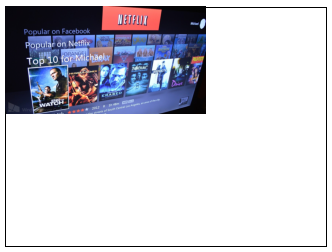
\includegraphics[width=\paperwidth]{general_figures/ml_intro_1}}}
\only<2>{\makebox[\linewidth]{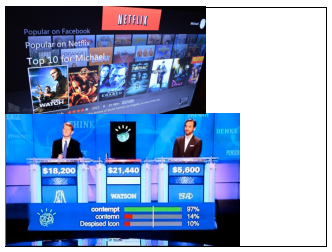
\includegraphics[width=\paperwidth]{general_figures/ml_intro_2}}}
\only<3>{\makebox[\linewidth]{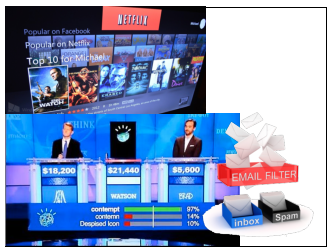
\includegraphics[width=\paperwidth]{general_figures/ml_intro_3}}}
\only<4>{\makebox[\linewidth]{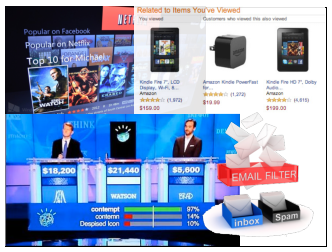
\includegraphics[width=\paperwidth]{general_figures/ml_intro_4}}}
\only<5>{\makebox[\linewidth]{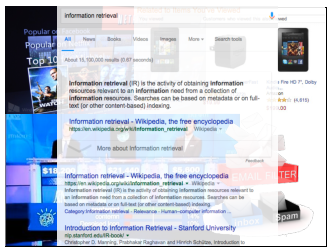
\includegraphics[width=\paperwidth]{general_figures/ml_intro_5}}}
\only<6>{\makebox[\linewidth]{
\includegraphics[width=\paperwidth]{general_figures/blackbox}}}
\only<7>{\makebox[\linewidth]{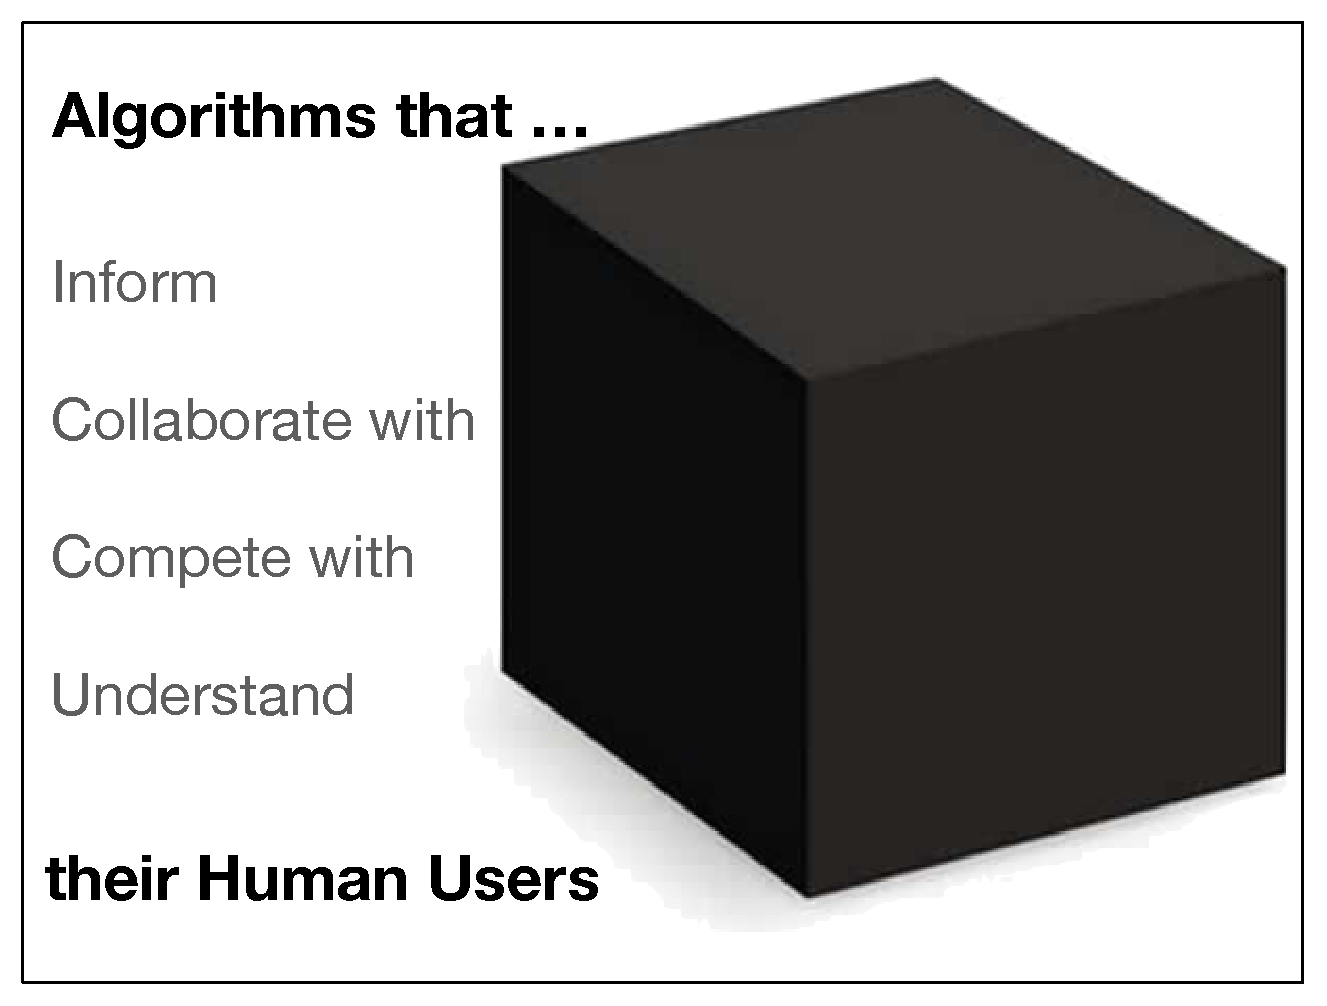
\includegraphics[width=\paperwidth]{general_figures/black_box_outline}}}
\only<8>{\makebox[\linewidth]{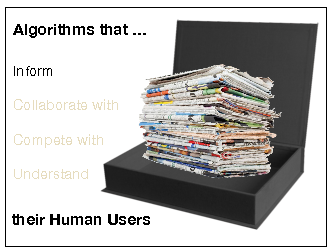
\includegraphics[width=\paperwidth]{general_figures/black_box_inform}}}
\end{frame}


\begin{frame}
\frametitle{The Challenge of Big Data}

\begin{columns}

\column{.5\linewidth}

Every second \dots
\begin{itemize}
  \item 600 new blog posts appear
  \item 34,000 tweets are tweeted
  \item 30 GB of data uploaded to Facebook
\end{itemize}
\pause

\begin{block}{Unstructured}
  No XML, no semantic web, no annotation.  Often just raw text.
\end{block}

\column{.5\linewidth}

\only<3->{
Common task: what's going on in this dataset.
\begin{itemize}
   \item Intelligence analysts
   \item Brand monitoring
   \item Journalists
   \item Humanists
\end{itemize}
}
\only<4>{
\centering
Common solution: topic models
}

\end{columns}

\end{frame}

\begin{frame}

\begin{center}
\frametitle{What does a Topic Model do?}
From an \textbf<1>{input corpus} and number of topics \textbf<1>{$K$} $\rightarrow$ \textbf<2>{words to topics} \\
\only<1>{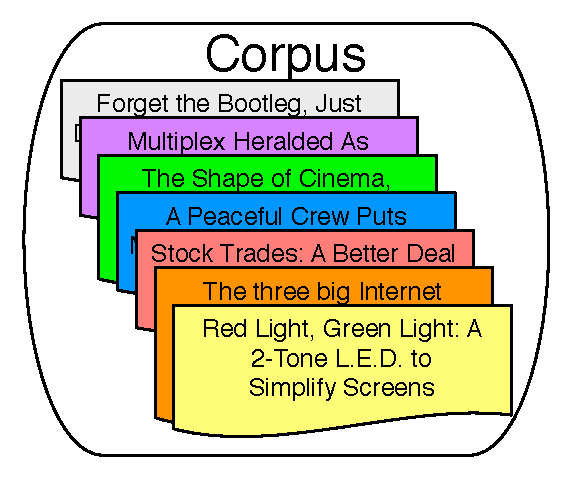
\includegraphics[width=0.6\linewidth]{reading_tea_leaves/figures/heldout_0} }
\only<2>{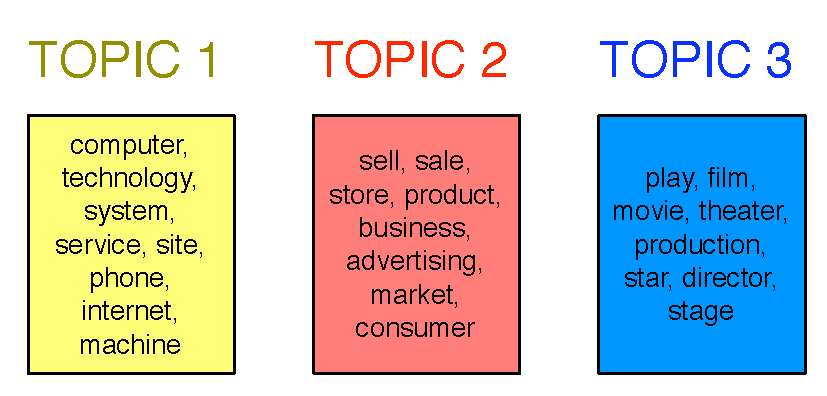
\includegraphics[width=0.9\linewidth]{reading_tea_leaves/figures/nyt_topics_wide}}
%\only<3>{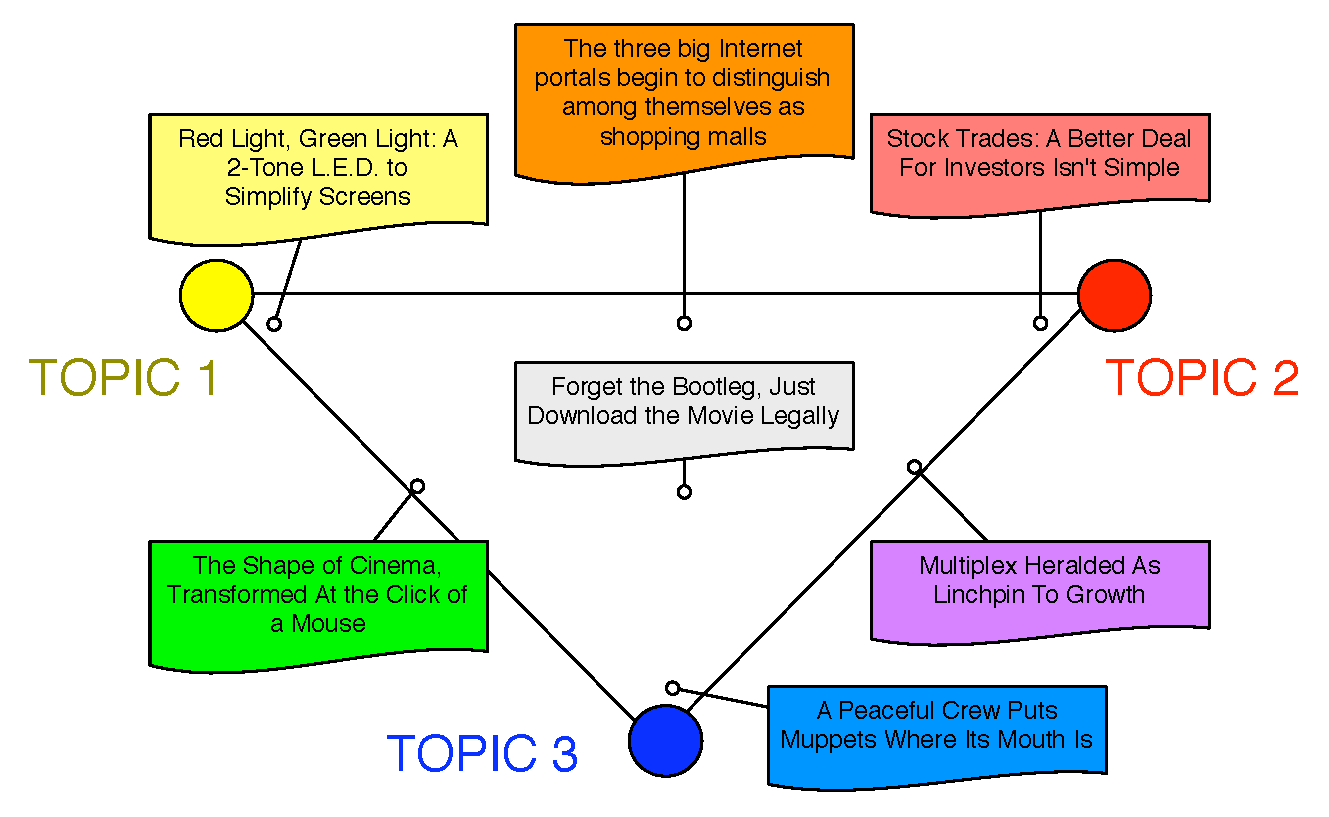
\includegraphics[width=0.9\linewidth]{topic_models/nyt_documents}}
\end{center}

\end{frame}


\begin{frame}{Evaluating Topic Models}

\begin{columns}

\column{.6\linewidth}
\begin{block}{ Reading Tea Leaves: How Humans Interpret Topic Models}
Jonathan Chang, Jordan Boyd-Graber, Chong Wang, Sean Gerrish, and David
M. Blei. Reading Tea Leaves: How Humans Interpret Topic Models. Neural
Information Processing Systems, 2009.
\end{block}

\ifjobtalk
{\bf Jonathan and I shared a NIPS 2009 Best Student Paper HM}
\fi

\column{.3\linewidth}
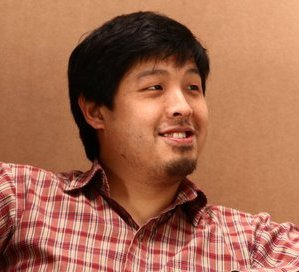
\includegraphics[width=.8\linewidth]{general_figures/jonathan}

\end{columns}

\end{frame}



\frame{
\frametitle{Evaluation}
\begin{center}
%\only<1>{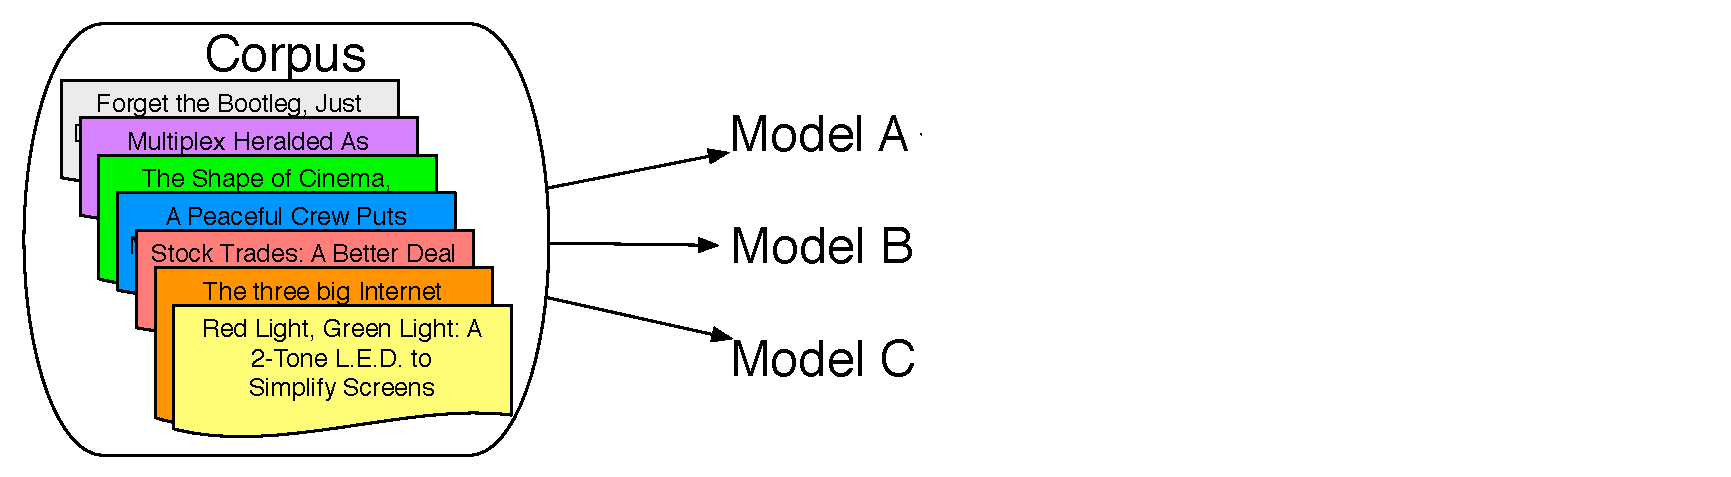
\includegraphics[width=0.9\linewidth]{reading_tea_leaves/figures/heldout_1} }
\only<1>{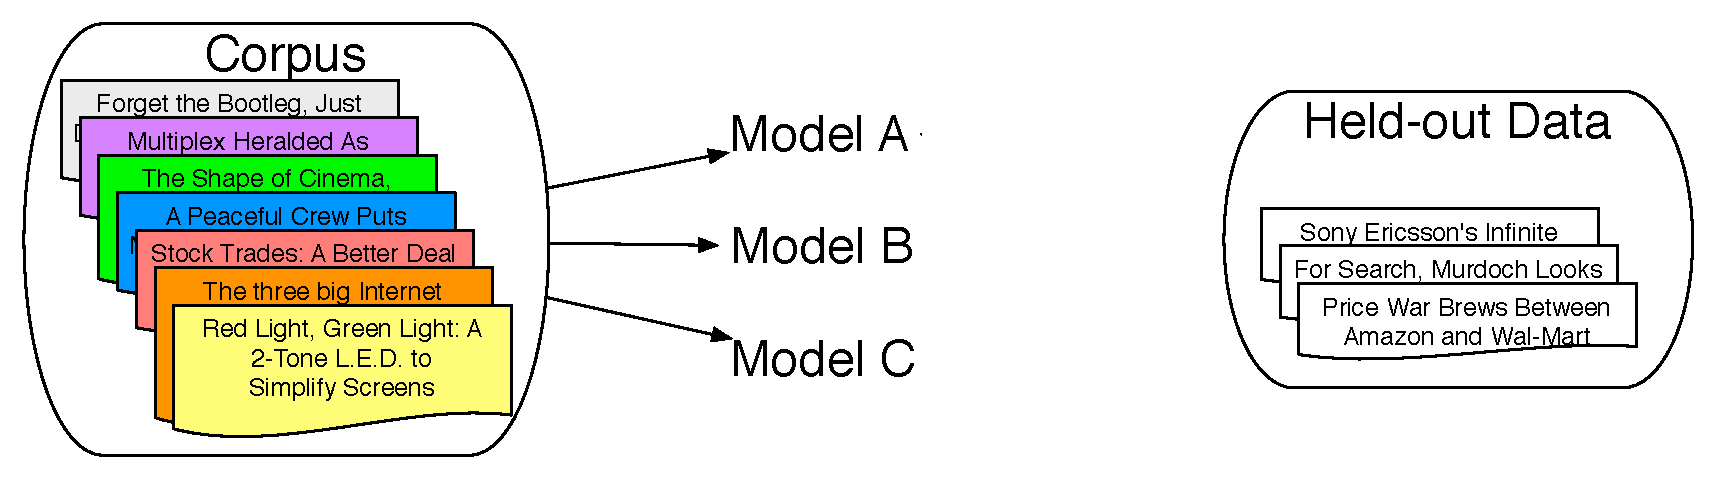
\includegraphics[width=\linewidth]{reading_tea_leaves/figures/heldout_2} }
%\only<3>{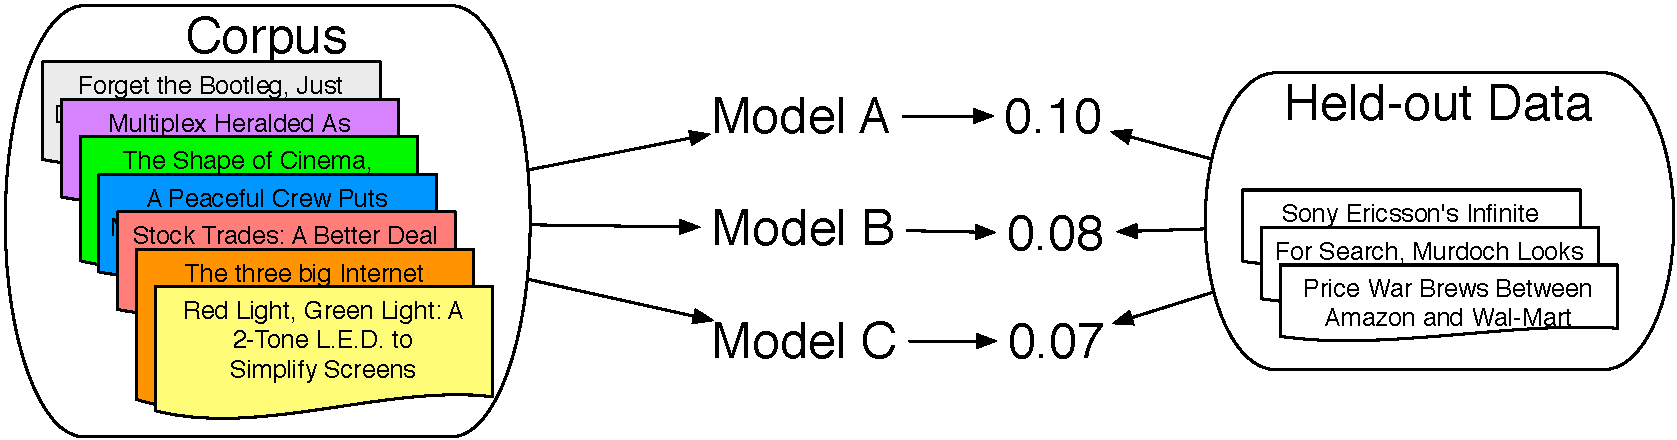
\includegraphics[width=\linewidth]{reading_tea_leaves/figures/heldout_3} }
\only<2>{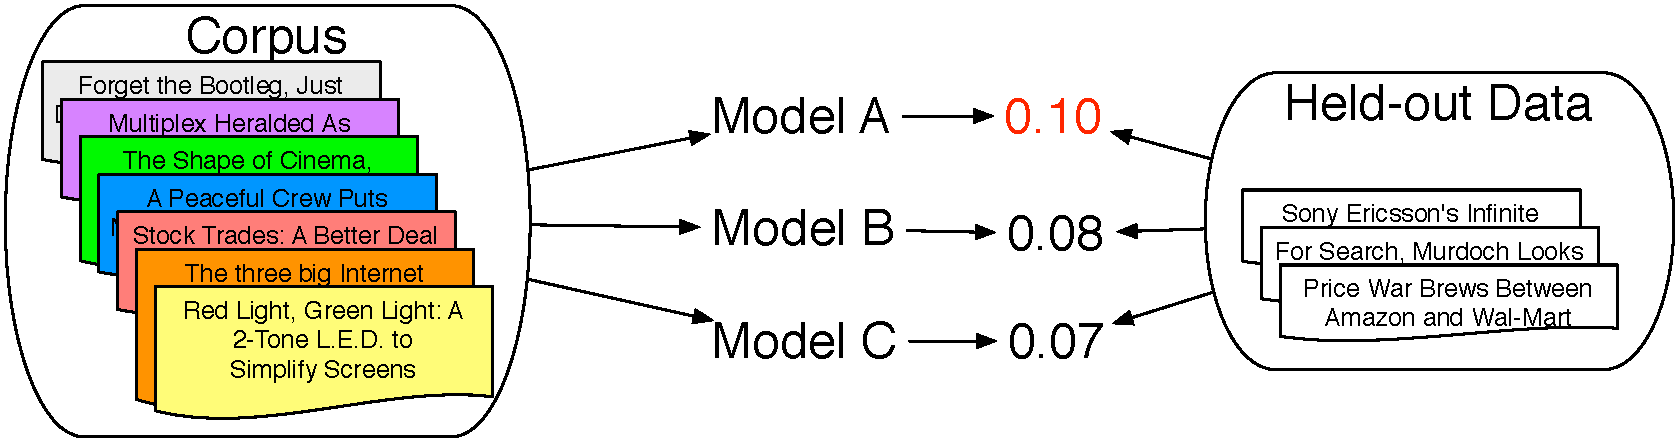
\includegraphics[width=\linewidth]{reading_tea_leaves/figures/heldout_4}  \\
	\large Measures predictive power (likelihood / perplexity)}
\end{center}
}


\frame{
        \frametitle{Interruption}

  \begin{columns}
  \column{.6\linewidth}
  \begin{block}{Do you have any real results?}
  \centering
     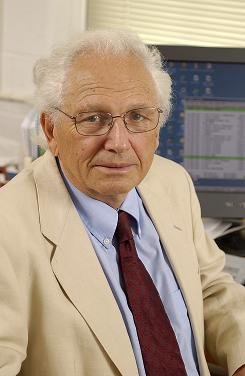
\includegraphics[width=0.5\linewidth]{reading_tea_leaves/jelinek} \\
     Fred Jelinek, inventor of perplexity~\cite{jelinek-76}
  \end{block}

  \column{.4\linewidth}

  \begin{itemize}
    \item Computational linguists and machine learning researchers like {\bf numbers}
    \item Likelihood and perplexity are convenient numbers
    \pause
    \item What do we {\bf actually} care about in topic models?
  \end{itemize}

  \end{columns}
}

\frame{
\frametitle{Qualitative Evaluation of the Latent Space}

\begin{center}
\only<1>{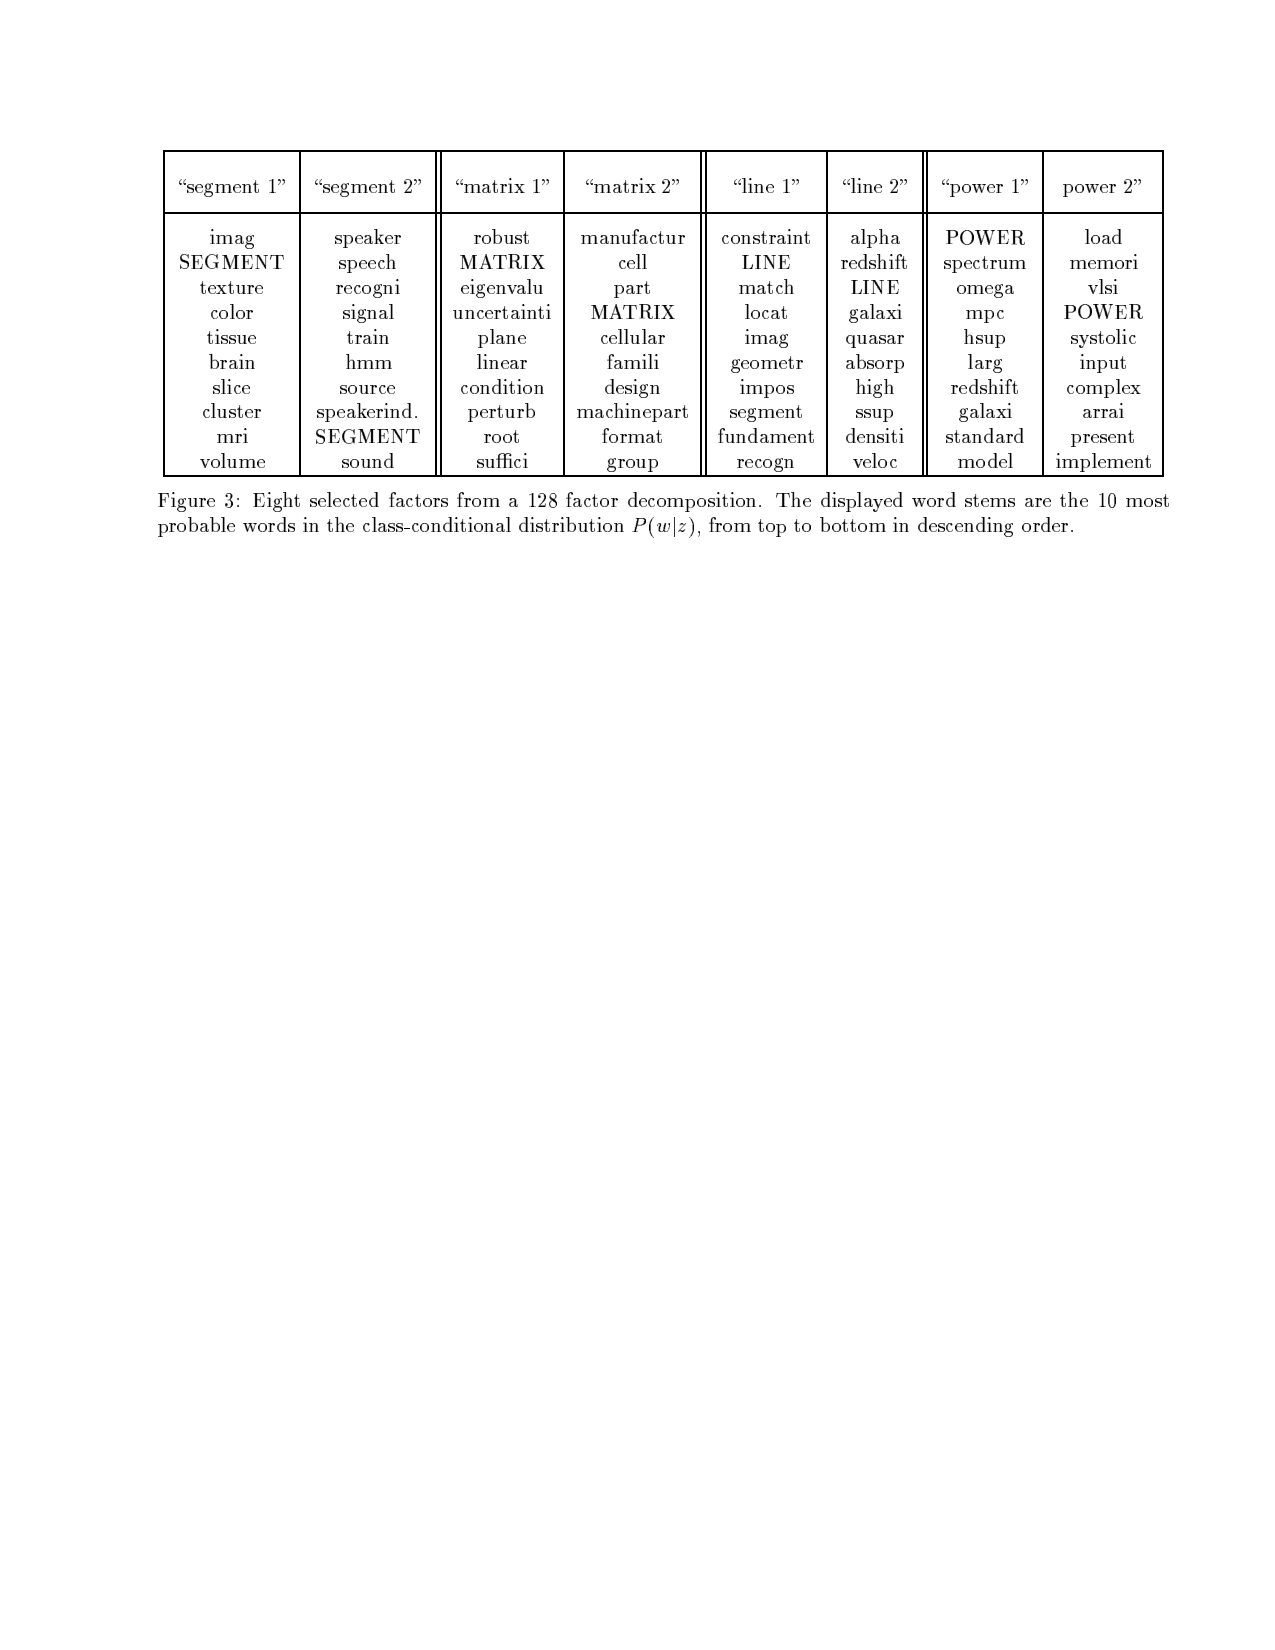
\includegraphics[width=0.9\linewidth]{reading_tea_leaves/topics_from_papers/1} \\ \cite{hofmann-99} }
\only<2>{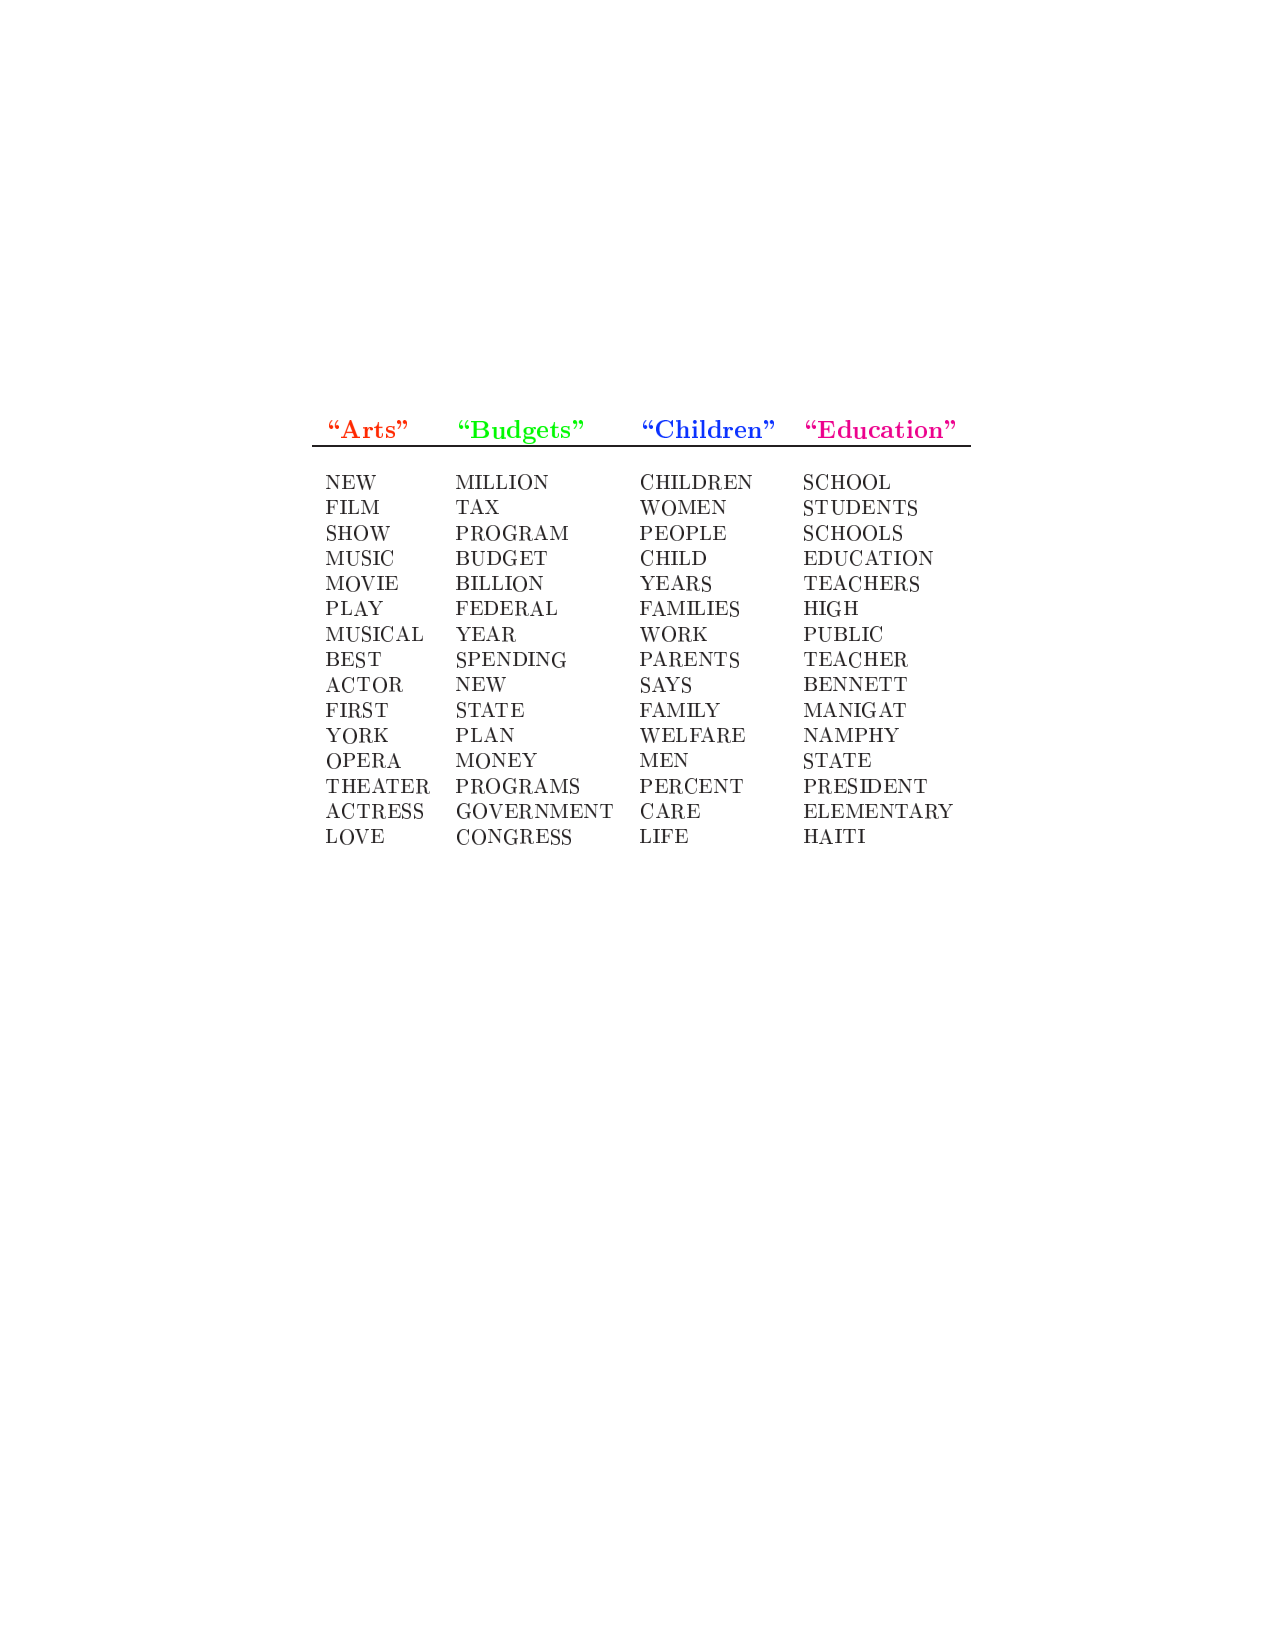
\includegraphics[width=0.7\linewidth]{reading_tea_leaves/topics_from_papers/2} \\ \cite{blei-03} }
\only<3>{
\includegraphics[width=0.7\linewidth]{reading_tea_leaves/topics_from_papers/3} \\ \cite{mimno-09} }
\only<4>{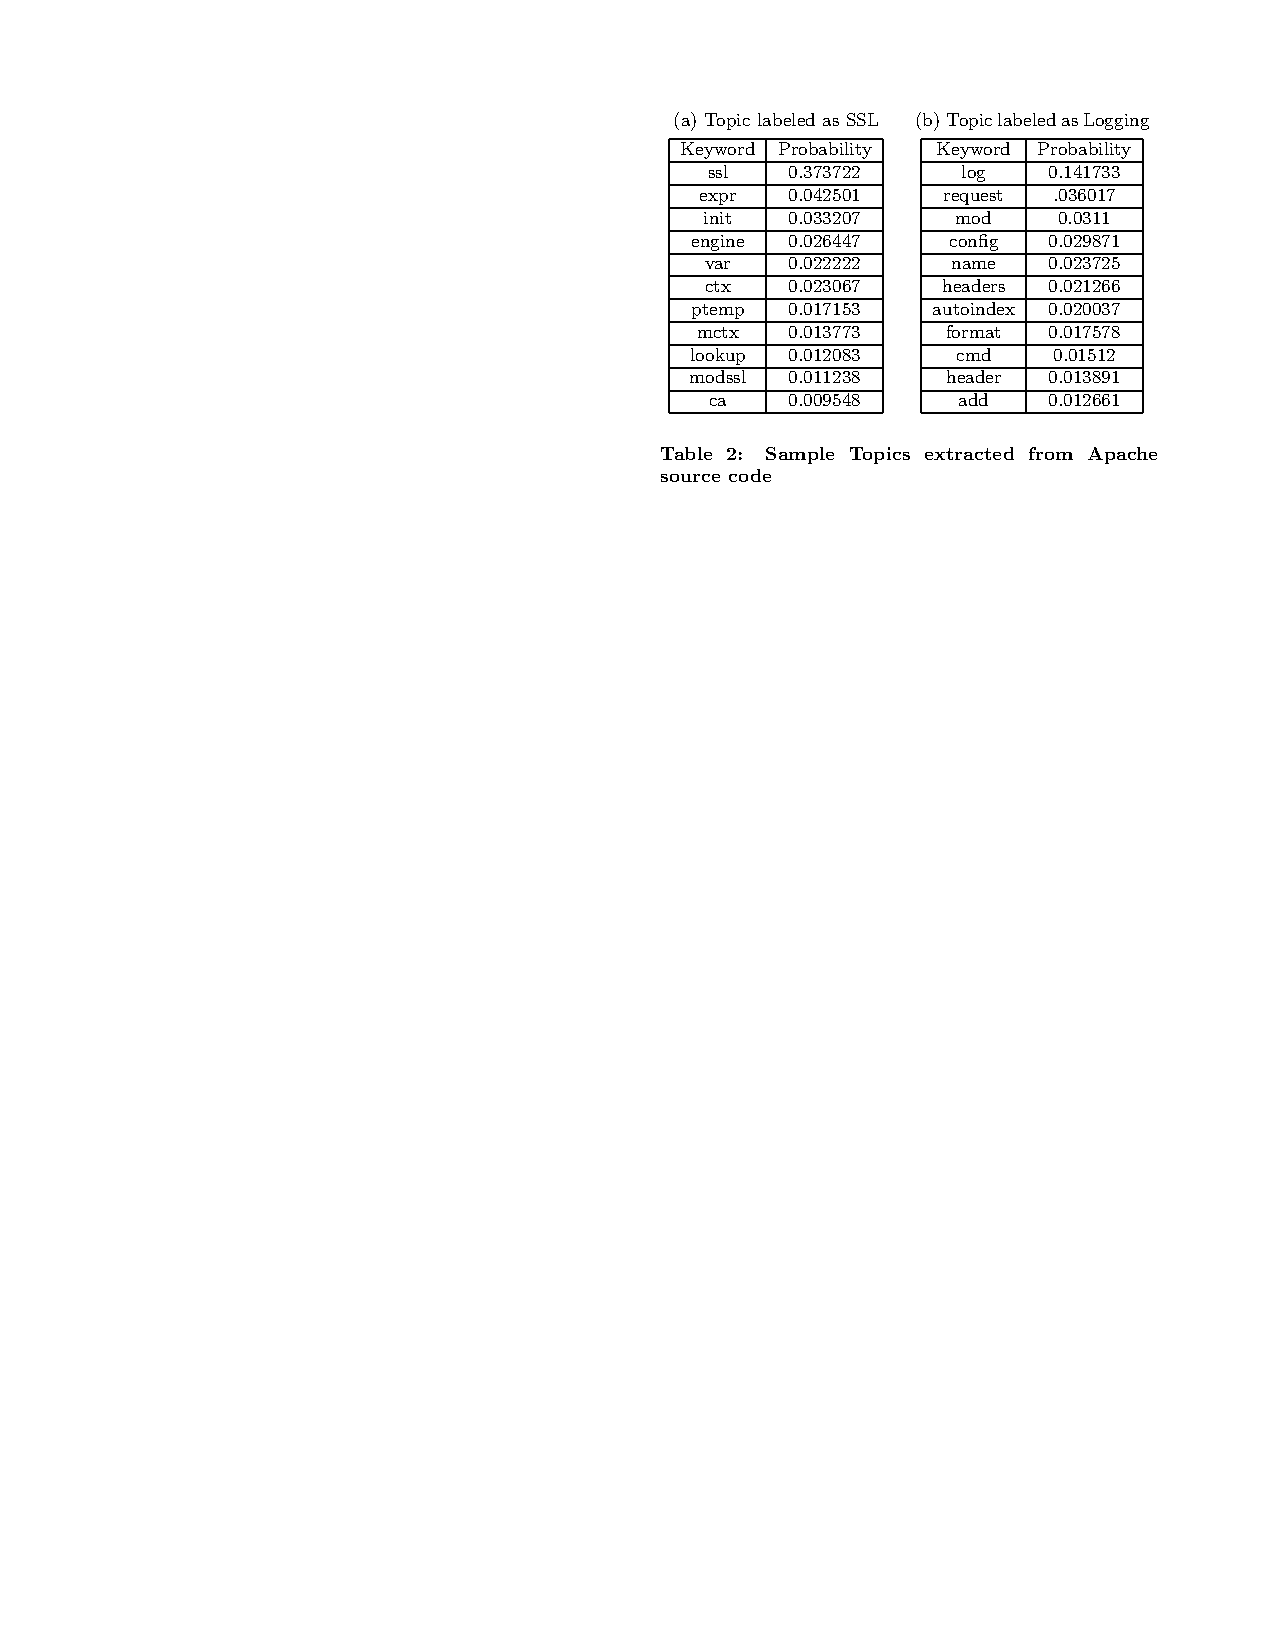
\includegraphics[width=0.7\linewidth]{reading_tea_leaves/topics_from_papers/4} \\ \cite{maskeri-08} }
\end{center}
}

\frame{
  \frametitle{Word Intrusion}

  \begin{enumerate}
    \item Take the highest probability words from a topic

      \begin{block}{Original Topic}
        dog, cat, horse, pig, cow
      \end{block}
\pause
    \item Take a high-probability word from another topic and add it
      \begin{block}{Topic with Intruder}
        dog, cat, \alert<2->{apple}, horse, pig, cow
      \end{block}
\pause
     \item We ask users to find the word that doesn't belong
  \end{enumerate}
\begin{block}{Hypothesis}
If the topics are interpretable, users will consistently choose true intruder
\end{block}
}


\frame{
\frametitle{Interpretability and Likelihood (NYT)}

\providecommand{\graphscale}{0.6}

\begin{columns}
\column{.84\linewidth}
  \only<1>{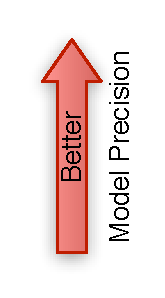
\includegraphics[scale=\graphscale]{reading_tea_leaves/tasks/mp}}
  \only<1>{
\includegraphics[scale=\graphscale]{reading_tea_leaves/tasks/mp_y}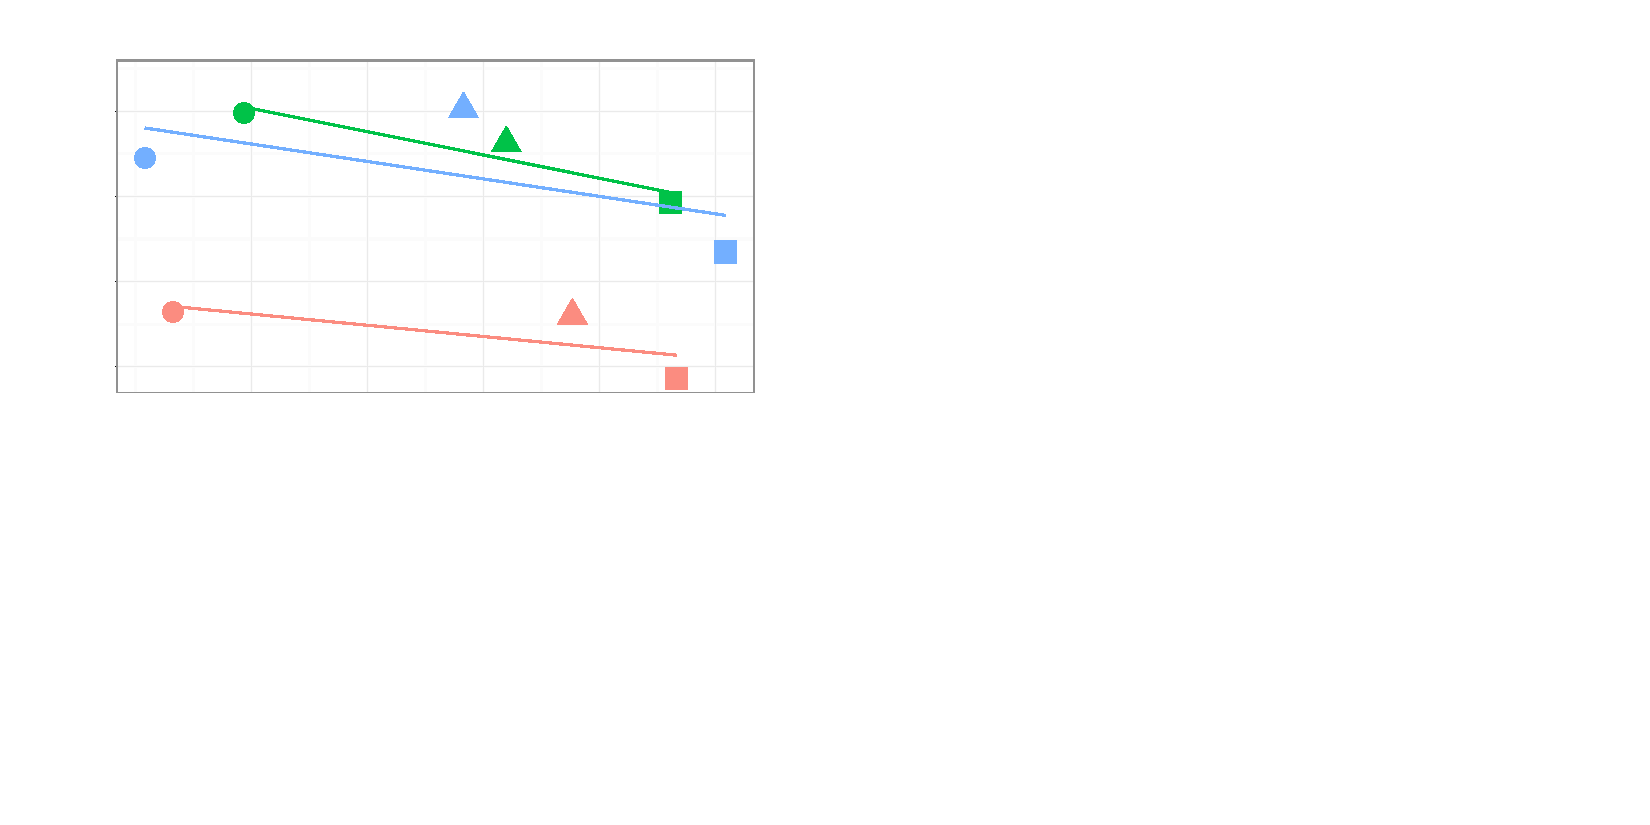
\includegraphics[scale=\graphscale]{reading_tea_leaves/tasks/nyt_mp}\\}
  \only<1>{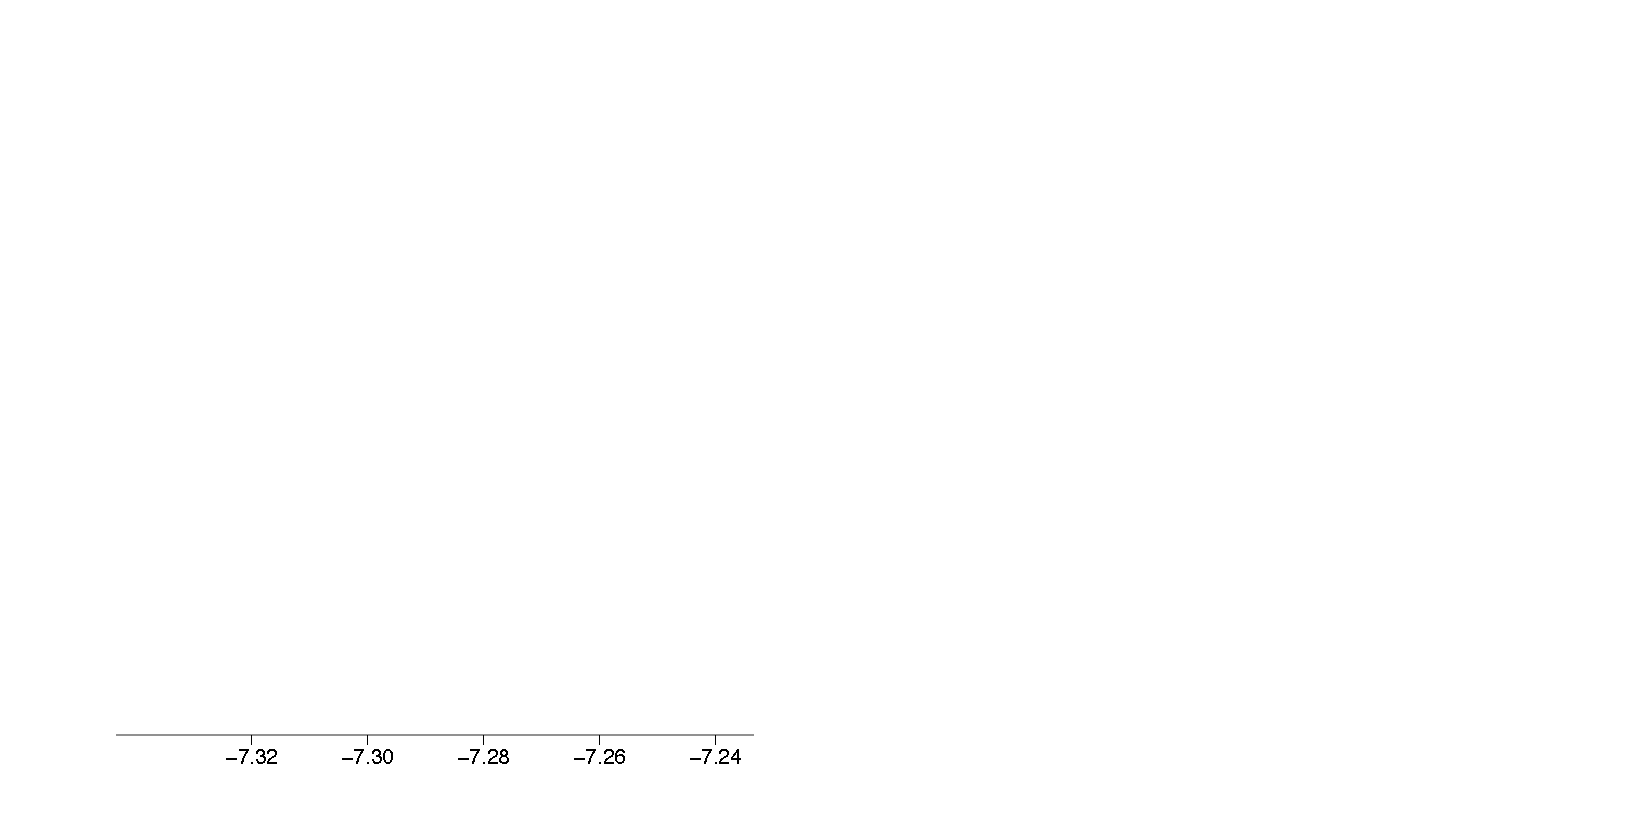
\includegraphics[scale=\graphscale]{reading_tea_leaves/tasks/nyt_x}}
\column{.15\linewidth}
  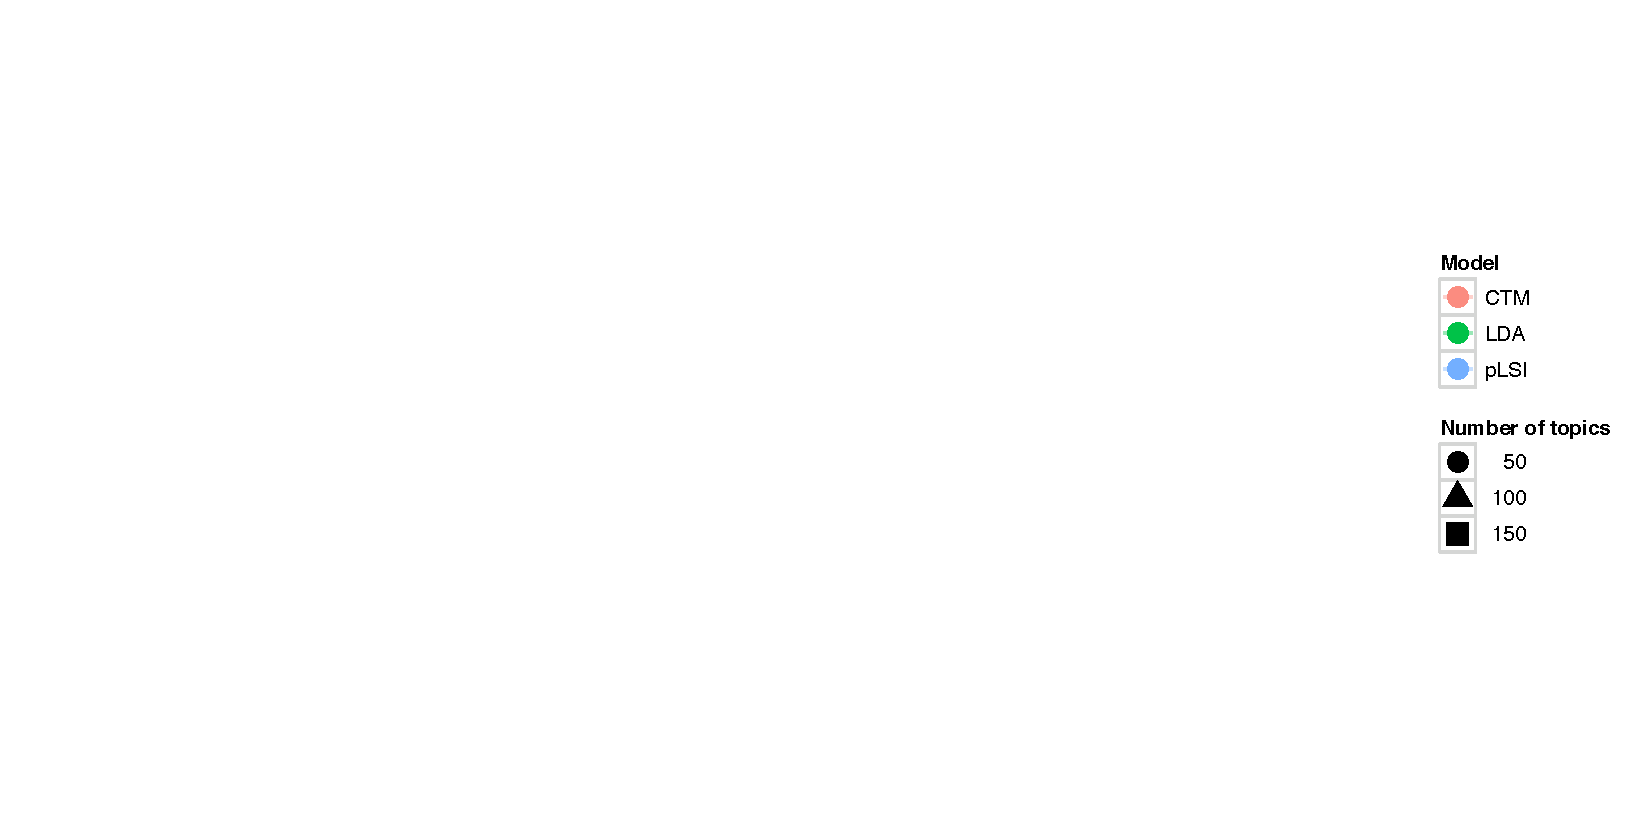
\includegraphics[scale=\graphscale]{reading_tea_leaves/tasks/legend}
\end{columns}

\begin{center}
  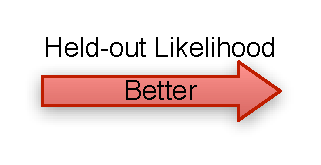
\includegraphics[scale=\graphscale]{reading_tea_leaves/tasks/held-out} \\
Within a model, higher likelihood $\not =$ higher interpretability
\end{center}
}


\begin{frame}{Since then \dots}

  \begin{itemize}
    \item A way to get at an evaluation that matches {\bf what we care about}
    \item A necessary step to improving topic models for navigating large datasets~\cite{talley-11}
    \item Others have discovered automatic methods that uncover the same properties~\cite{newman-10,mimno-11}
    \item And extended the technique to structured topics and phrases~\cite{lindsey-12,weninger-12}
  \end{itemize}

\end{frame}


\begin{frame}[plain]
\vspace*{-1pt}
\makebox[\linewidth]{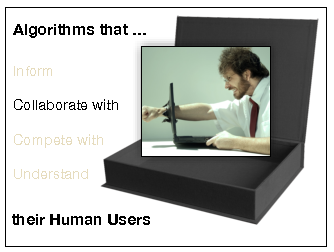
\includegraphics[width=\paperwidth]{general_figures/black_box_collaborate}}
\end{frame}

\frame{

\frametitle{The Problem: User Perspective}

\begin{columns}

\column{.4\linewidth}
\begin{center}
\begin{tabular}{ccc}
& \only<2->{\itmspace}\color<2->{red}{bladder} & \\
& \only<3->{\hspace{-2cm}} \color<3->{blue}{spinal\_cord}  & \\
& \only<3->{\hspace{-2cm}} \color<3->{blue}{sci} & \\
& \only<3->{\hspace{-2cm}}\color<3->{blue}{spinal\_cord\_injury} & \\
& \only<3->{\hspace{-2cm}}\color<3->{blue}{spinal} & \\
& \only<2->{\itmspace}\color<2->{red}{urinary} & \\
& \only<2->{\itmspace}\color<2->{red}{urothelial} & \\
& \only<3->{\hspace{-2cm}}\color<3->{blue}{cervical} & \\
& injury & \\
& recovery & \\
& \only<2->{\itmspace}\color<2->{red}{urinary\_tract} & \\
& locomotor & \\
& \only<3->{\hspace{-2cm}}\color<3->{blue}{lumbar} & \\
\end{tabular}
\end{center}

\column{.6\linewidth}

\danquote{These words don't belong together!}

\end{columns}

}


\begin{frame}
  \frametitle{Adding meaning to topic models}
        \begin{block}{Traditional Topic Models}
                $ p(w) = \prod_d \prod_n^{N_d} \left( p(w_{d,n} | \phi_{z_{d,n}})
                  \explain{\alert<3>{topic}}{p(z_{d,n} | \theta_d)} \right) p(\theta_d | \alpha)                 \explain{\alert<2>{topic to words}}{ \prod_k^K
p(\phi_k | \eta) }$
        \end{block}

        \begin{block}{Our Model}
          \vspace{-0.8cm}
          \begin{align*}
               p(w) = \prod_d \prod_n^{N_d} & \left( p(w_{d,n} | \pi_{l_{d,n}})
                 \explain{\alert<6>{meaning and topic}} {p(l_{d,n} | \phi_{d,n} )
                   p(z_{d,n} | \theta_d)}  \right) p(\theta_d | \alpha) \\
               &  \explain{\alert<4>{topic to concept}}{\prod_k^K
                p(\phi_k | \eta)} \explain{\alert<5>{concept to word}}{\prod_c^C \left(
                  p(\pi_{k,c} | \tau) \right) }
           \end{align*}
        \end{block}


\end{frame}



\providecommand{\tb}[1]{\parbox{0.8\linewidth}{ \tiny{ #1 }} \vspace{.2cm} }

\frame{

\vspace{-1cm}

\begin{columns}

\column{.5\linewidth}

\begin{tabular}{l*{2}{c}r}
	Topic & Before \\
\hline

\alert<2>{{\bf 1}} & \tb{ \alert<2>{election, yeltsin, russian, political, party, democratic, russia,
  president, democracy, boris, country, south, years, month, government, vote,
  since, leader, presidential, military} } \\

2 & \tb{new, york, city, state, mayor, budget, giuliani, council, cuomo, gov,
  plan, year, rudolph, dinkins, lead, need, governor, legislature, pataki,
  david} \\

3 & \tb{nuclear, arms, weapon, defense, treaty, missile, world, unite, yet,
  soviet, lead, secretary, would, control, korea, intelligence, test, nation,
  country, testing} \\

4 & \tb{president, bush, administration, clinton, american, force, reagan, war,
  unite, lead, economic, iraq, congress, america, iraqi, policy, aid,
  international, military, see} \\

& \vdots \\

\alert<2>{{\bf 20}} & \tb{\alert<2>{soviet, lead, gorbachev, union, west, mikhail, reform, change, europe,
  leaders, poland, communist, know, old, right, human, washington, western,
  bring, party} }\\

\end{tabular}

\column{.5\linewidth}

\only<3> {

	\begin{block}{Suggestion}
	\emph{boris, communist, gorbachev, mikhail, russia,
  russian, soviet, union, yeltsin }
	\end{block}

}

\only<4-> {

\begin{tabular}{l*{2}{c}r}
	Topic & After \\
\hline

\alert<5>{{\bf 1}} & \alert<5>{\tb{election, democratic, south, country, president, party, africa, lead,
  even, democracy, leader, presidential, week, politics, minister, percent,
  voter, last, month, years} } \\

\alert<6>{2} & \tb{new, york, city, state, mayor, budget, council, giuliani, gov, cuomo,
  year, rudolph, dinkins, legislature, plan, david, governor, pataki, need, cut}
\\

\alert<6>{3} & \tb{nuclear, arms, weapon, treaty, defense, war, missile, may, come, test,
  american, world, would, need, lead, get, join, yet, clinton, nation} \\

\alert<6>{4} & \tb{president, administration, bush, clinton, war, unite, force, reagan,
  american, america, make, nation, military, iraq, iraqi, troops, international,
  country, yesterday, plan} \\

   & \vdots \\

\alert<4>{ {\bf 20} } & \alert<4> {\tb{soviet, union, economic, reform, yeltsin, russian, lead, russia,
  gorbachev, leaders, west, president, boris, moscow, europe, poland, mikhail,
  communist, power, relations} } \\

\end{tabular}

}

\end{columns}

}


\providecommand{\blue}[1]{{\color{blue}{#1}}}
\providecommand{\red}[1]{{\color{red}{#1}}}
\providecommand{\green}[1]{{\color{green}{#1}}}

\begin{frame}

\frametitle{Example: Negative Constraint}

\begin{columns}

\column{.4\linewidth}

\begin{tabular}{l*{2}{c}r}
	Topic & Words \\
\hline

{\bf 318} & \tb{\red{bladder}, sci, \blue{spinal\_cord}, \blue{spinal\_cord\_injury}, \blue{spinal}, \red{urinary}, \red{urinary\_tract}, \red{urothelial},\blue{injury}, \blue{motor}, \blue{recovery}, \blue{reflex}, \blue{cervical}, \red{urothelium}, \blue{functional\_recovery}} \\

\end{tabular}

\column{.1\linewidth}

\column{.4\linewidth}

\only<3->{
\begin{tabular}{l*{2}{c}r}
	Topic & Words \\
\hline

{\bf 318} & \tb{sci, \blue{spinal\_cord}, \blue{spinal\_cord\_injury}, \blue{spinal}, \blue{injury}, \blue{recovery}, \blue{motor}, \blue{reflex}, \red{urothelial}, \green{injured}, \blue{functional\_recovery}, \green{plasticity}, \green{locomotor}, \blue{cervical}, \green{locomotion}}\\

\end{tabular}
}

\end{columns}

\only<2->{
\begin{block}{Negative Constraint}
  spinal\_cord, bladder
\end{block}

}

\end{frame}



\begin{frame}{Real-World Use Cases}

  \begin{itemize}
    \item GSA
    \item NSF
    \item FCC
   \end{itemize}

\end{frame}

\begin{frame}[plain]
\vspace*{-1pt}
\makebox[\linewidth]{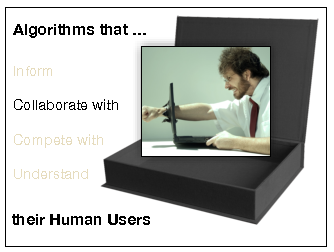
\includegraphics[width=\paperwidth]{general_figures/black_box_collaborate}}
\end{frame}

\begin{frame}[plain]{}
\vspace*{-4cm}
 \gfxs{nuremberg_trials}{1.0}

\vspace{-4cm}

\begin{block}{N\"urnberg Trials}
    \begin{itemize}
        \item Dozens of defendants
        \item Judges from four nations (three languages)
        \item Status quo: speak, then translate
     \end{itemize}

\end{block}


\end{frame}


\section{Simultaneous Translation}

\begin{frame}{Simultaneous translation now the norm}

  \begin{columns}
    \column{.5\linewidth}
       \gfxs{nuremberg_translators}{.9}
    \column{.5\linewidth}
       \begin{itemize}
         \item Rigorous training
         \item Technological sophistication
         \item Long way from ``sentence at a time''
       \end{itemize}
  \end{columns}

\end{frame}

\begin{frame}{Why interpretation really hard is}

  \begin{columns}
    \column{.5\linewidth}
      \begin{itemize}
        \item Many languages are \textsc{sov}
        \item \alert<2>{German}, Japanese, Farsi, Korean,
          \alert<3>{Yiddish}
        \item<4-> How can we learn from trained interpreters?
      \end{itemize}
    \column{.5\linewidth}
      \gfxs{yoda}{.6}
  \end{columns}

  \centering

\only<4-5>{
\vspace{1cm}

\begin{tabular}{c@{ }c@{ }c@{ }c@{ }c@{ }c@{ }c@{ }l}
ich & bin & mit & dem & Zug & nach & Ulm & {\bf gefahren} \\
I & am & with & the & train & to & Ulm & {\bf traveled} \\
\hline
I & \multicolumn{6}{c}{\emph{(\dots\dots waiting\dots\dots)}} & {\bf traveled} by train to Ulm \\
\end{tabular}
}

\only<6>{
  \gfxs{en_ja_example}{.8}
}

\end{frame}

\begin{frame}[plain]{}
\vspace*{-1pt}
  \gfxs{interpreter-screenshot}{1.0}

  \pause
  \vspace{-4cm}

  \begin{block}{Learning from Interpreters}
    \begin{itemize}
      \item What tricks do they use?
      \item How can we teach machines to use them?
      \item How do we know when to use them?
      \item Giving back to interpreters
    \end{itemize}
  \end{block}

\end{frame}

\begin{frame}{What tricks to interpreters use?}

  \begin{columns}
    \column{.5\linewidth}
  \begin{itemize}
    \item Generalize~\cite{dell92access,cuetos06access}
    \item Summarize
    \item Passivization
    \item Segmentation~\cite{erik11theory,shimizu13iwslt}
    \item Predictions~\cite{levy2013expectation,momma2015timing}
  \end{itemize}
    \column{.5\linewidth}
    \centering
        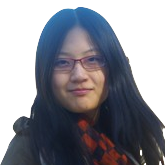
\includegraphics[width=0.4\linewidth]{general_figures/hehe}
        \begin{block}{ {\bf \href{http://cs.colorado.edu/~jbg/docs/2016_naacl_interpretese.pdf}{Interpretese vs. Translationese: The Uniqueness of Human Strategies in Simultaneous Interpretation}}}
He He, {\bf Jordan Boyd-Graber}, and Hal {Daum\'{e} III}.
\emph{North American Association for Computational Linguistics}, 2016
        \end{block}
  \end{columns}


  % Need pictures / examples

\end{frame}



\begin{frame}{}

  \begin{columns}
    \column{.5\linewidth}
        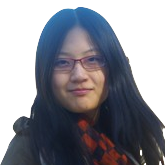
\includegraphics[width=0.8\linewidth]{general_figures/hehe}
    \column{.5\linewidth}
        \begin{block}{ {\bf \href{http://cs.colorado.edu/~jbg//docs/2015_emnlp_rewrite.pdf}{Syntax-based Rewriting for Simultaneous Machine Translation}}}
He He, Alvin Grissom II, {\bf Jordan Boyd-Graber}, and Hal {Daum\'{e} III}.  \emph{Empirical Methods in Natural Language Processing}, 2015
        \end{block}
  \end{columns}
\end{frame}

\begin{frame}{How can we make MT better?}

  \gfxs{en_ja_example}{.9}

  \pause

  \begin{itemize}
    \item In a perfect world, we'd use interpretation data
      \pause
      \item Very rare, and low quality in other ways
      \pause
    \item But can we \emph{rewrite} batch translations?
  \end{itemize}

\end{frame}

\begin{frame}{Are there enough opportunities?}


\begin{center}
\begin{tabular}{lcccc}
\toprule
& \alert<2>{verb} & \alert<3>{voice} & \alert<4>{noun} & \alert<5>{clauses} \\
\midrule
Applicable \% & \only<2->{39.9} & \only<3->{50.0} & \only<4->{26.4} & \only<5->{4.8} \\
Accepted \% & \only<2->{22.5} & \only<3->{24.0} & \only<4->{51.2} & \only<5->{38.4} \\
\bottomrule
\end{tabular}
\end{center}

\only<2>{
\begin{itemize*}
\item[O:] {\bf They announced} that the president will restructure the division.
\item[R:] The president will restructure the division, {\bf they announced}.
\end{itemize*}
}


\only<3>{
  \begin{columns}
    \column{.4\linewidth}

    \gfxs{rewrite_input}{.9}
    \column{.55\linewidth}
    \vspace{-.5cm}
    \gfxs{rewrite_transform}{.9}
   \end{columns}
}

\only<4>{
\begin{itemize*}
  \item[O:] the e-mail server of Clinton
  \item[R:] Clinton's e-mail server
\end{itemize*}
}

\only<5>{
\begin{itemize*}
\item[O:] \pos{S}$_1$ \pos{conj} \pos{S}$_2$: We should march {\bf because} winter is coming.
\item[O:] \pos{conj} \pos{S}$_2$, \pos{S}$_1$: {\bf Because} winter is
  coming, we should march.
\vspace{1cm}
\item[R:] \pos{S}$_2$, \pos{conj'} \pos{S}$_1$: Winter is coming, {\bf because of this}, we should march.
\end{itemize*}
}


\end{frame}

\begin{frame}{}

\gfxs{rewrite_eval}{.8}
\pause
We rewrite 32.2\% of
sentences, reducing the delay from 9.9 words/seg to 6.3 words/seg per
segment for rewritten sentences and from 7.8 words/seg to 6.7 words/seg overall.

\end{frame}

\begin{frame}{How good are the translations?}

  \gfxs{tradeoff-rw-bleu}{.7}

\begin{center}
Aggressiveness based on different right probability thresholds
\cite{fujita-13}
\end{center}

\end{frame}

\begin{frame}{Why does the quality improve?}

\begin{center}
\begin{tabular}{ccccc}
\toprule
& \multicolumn{3}{c}{Translation} & \\
\cmidrule{2-4}
& \abr{gd} & \abr{rw} & \abr{rw+gd} & Gold ref \\
\midrule
\# of verbs & 1971 & 2050 & {\bf 2224} & 2731 \\
\bottomrule
\end{tabular}
\end{center}

\end{frame}


\begin{frame}{}

  \begin{columns}
    \column{.5\linewidth}
        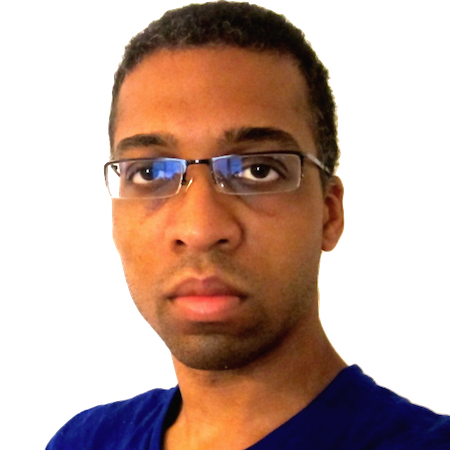
\includegraphics[width=0.9\linewidth]{general_figures/alvin}
    \column{.5\linewidth}
        \begin{block}{ {\bf \href{http://cs.colorado.edu/~jbg//docs/2014_emnlp_simtrans.pdf}{Don't Until the Final Verb Wait: Reinforcement Learning for Simultaneous Machine Translation}}}
\underline{\href{http://www.umiacs.umd.edu/~alvin/}{Alvin Grissom II}}, {\bf Jordan Boyd-Graber}, He He, John Morgan, and Hal {Daum\'{e} III}.  \emph{Empirical Methods in Natural Language Processing}, 2014
        \end{block}
  \end{columns}
\end{frame}

\begin{frame}[plain]
\vspace{-4cm}
\gfxs{autocomplete}{1.0}
\pause
\vspace{-6cm}
\begin{block}{Predict the Verb}
  \begin{itemize}
    \item Predicting the verb ``unlocks'' sentence
    \item Language models are good at word prediction
    \item But instead, we'll predict the verb
  \end{itemize}
\end{block}

\end{frame}


\begin{frame}{Language Models of Verbs}

  \only<1>{\gfxs{verb_corpus_1}{.9}}
  \only<2>{\gfxs{verb_corpus_2}{.9}}
  \only<3>{\gfxs{verb_corpus_3}{.9}}

\end{frame}

\begin{frame}{Predicting the Verb}
\begin{itemize}
  \item Build language model for every verb
  \item Then, for any input text $x$ we can make a prediction of the verb
\begin{equation}
  \arg\max_v p(v) \prod_{i=1}^t p(x_i \g v, x_{i-n+1:i-1})
\end{equation}
\pause
  \item Most of these predictions will be totally wrong (18\%
    accuracy) \dots
  \item leading to horrible translations
\end{itemize}
\end{frame}

% \begin{frame}{Consensus Translation}

%   \only<1>{\begin{center}
% ``German in, English out'' black box
%       \end{center}}

%   \only<2>{\gfxs{consensus_0}{.8}}
%   \only<3>{\gfxs{consensus_1}{.8}}
%   \only<4>{\gfxs{consensus_2}{.8}}
%   \only<5>{\gfxs{consensus_3}{.8}}
%   \only<6>{\gfxs{consensus_4}{.8}}

% \end{frame}

\begin{frame}{Scoring one Translation}
  \begin{center}
    Bilingual Evaluation Understudy (BLEU)
\end{center}
  \only<1>{\gfxs{bleu_ex}{.8}}
  \only<2>{\gfxs{bleu_correlation}{.6}}
\end{frame}


\begin{frame}{Scoring a series of Translations}
  \begin{center}
    Bilingual Evaluation Understudy (BLEU)
\end{center}
  \only<1>{\gfxs{integral_0}{.95}}
  \only<2>{\gfxs{integral_1}{.95}}
\end{frame}



\begin{frame}{Comparing Policies}

  \only<1-7>{\vspace{4.75cm}}
  \only<8-14>{\vspace{3.3cm}}
  \only<15-21>{\vspace{2cm}}

  \only<1,8,15,22>{\gfxs{reward_example_0}{.8}}
  \only<2,9,16,23>{\gfxs{reward_example_1}{.8}}
  \only<3,10,17,24>{\gfxs{reward_example_2}{.8}}
  \only<4,11,18,25>{\gfxs{reward_example_3}{.8}}
  \only<5,12,19,26>{\gfxs{reward_example_4}{.8}}
  \only<6,13,20,27>{\gfxs{reward_example_5}{.8}}
  \only<7,14,21,28>{\gfxs{reward_example_6}{.8}}
\end{frame}




\begin{frame}{Imitation Learning}

  \begin{columns}
    \column{.5\linewidth}
       \gfxs{imitation_fold}{.8}
       \gfxs{imitation_drive}{.8}
    \column{.5\linewidth}
    \begin{itemize}
      \item Given all the predictions that we make (and the resulting
        translations) \dots
      \item Discover the optimal in hindsight policies
      \item Goal: Teach our algorithm to think on its feet
      \item Challenge: Represent states in a way that will generalize
    \end{itemize}

  \end{columns}

\end{frame}


\begin{frame}{How do we find a good policy?}

\only<1>{\gfxs{searn_1}{1.0}}
\only<2>{\gfxs{searn_2}{1.0}}
\only<3>{\gfxs{searn_3}{1.0}}
\only<4>{\gfxs{searn_4}{1.0}}
\only<5>{\gfxs{searn_5}{1.0}}
\only<6>{\gfxs{searn_6}{1.0}}
\only<7>{\gfxs{searn_7}{1.0}}
\only<8>{\gfxs{searn_8}{1.0}}
\only<9>{\gfxs{searn_9}{1.0}}
\end{frame}


\begin{frame}{How do we find a good policy?}

  \begin{itemize}
    \item Find optimal policies through dynamic programming $\pi_0
      \equiv \pi*$
    \item Represent states $s$ through a feature vector $\vec f(s)$
      \pause
    \item Until convergence:
      \begin{itemize}
        \item Generate examples of state action pairs: $(\pi_t(s), s)$
        \item Create a classifier that maps states to actions (an
          apprentice policy) $h_t: f(s) \mapsto A$ \only<3->{(Loss of
            classifier is the negative reward)}
    \item Interpolate learned classifier $\pi_{t+1} = \lambda \pi_t +
      (1-\lambda) h_t$
  \end{itemize}
  \end{itemize}

\only<4->{
  \begin{center}
    \textsc{searn}: \underline{Se}arching to L\underline{earn}
    (Daum\'e \& Marcu, 2006)
    \end{center}
}
\end{frame}


\begin{frame}{Experimental Setup}

  \begin{itemize}
    \item \textsc{denews} corpus
      \begin{itemize}
        \item News snippets
        \item Some formulaic
        \item Some surprising
      \end{itemize}
    \item Only verb-final sentences
    \item Some compromises with translation system (to make sure verbs appeared)
  \end{itemize}

\end{frame}



\begin{frame}{Comparing Policies}

  \gfxs{cummulative}{.6}

\end{frame}

\begin{frame}{Learned Policy with Accumulated Reward}

  \only<1>{\gfxs{compare_line_batch}{.8}}
  \only<2>{\gfxs{compare_line_batch_monotone}{.8}}
  \only<3>{\gfxs{compare_line_batch_monotone_opt}{.8}}
  \only<4>{\gfxs{compare_line_all}{.8}}
\end{frame}


\begin{frame}{Example Sentence}

  \gfxs{ex_imperfect}{.7}

\end{frame}

\begin{frame}[plain]

\only<1>{ \gfxs{computer-interpreter}{1.0} }
\only<2>{ \gfxs{computer-interpreter}{1.0}
\vspace{-5cm}
\gfxs{centaur-chess}{0.8}}

\end{frame}


\begin{frame}[plain]
\vspace*{-1pt}
\makebox[\linewidth]{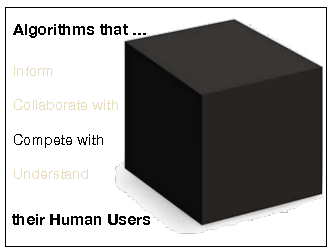
\includegraphics[width=\paperwidth]{general_figures/black_box_compete}}
\end{frame}


\section{Quiz Bowl}

\begin{frame}[plain]
  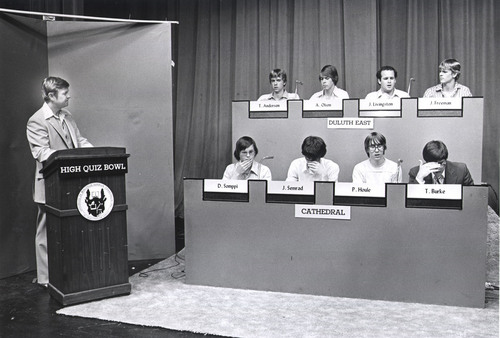
\includegraphics[width=1.0\linewidth]{qb/quizbowl}
\end{frame}

\begin{frame}[t]
\frametitle{Sample Question}
	\frametitle{Sample Question}

With Leo Szilard, he invented a doubly-eponymous \only<2->{refrigerator with no moving parts. He did not take interaction with neighbors into account when formulating his theory of} \only<3->{heat capacity, so} \only<4->{Debye adjusted the theory for low temperatures. His} \only<4->{summation convention automatically sums repeated indices in tensor products. His name is attached to the A and B coefficients} \only<5->{for spontaneous and stimulated emission, the subject of one of his multiple groundbreaking 1905 papers. He further developed the model of statistics sent to him by} \only<6->{Bose to describe particles with integer spin. For 10 points, who is this German physicist best known for formulating the} \only<7->{special and general theories of relativity?} \\
\vspace{1cm}
\only<8->{ {\bf Albert \underline{Einstein}}}

\ifjobtalk
\only<9->{
\vspace{-6cm}

\begin{block}{Faster = Smarter}

  \begin{enumerate}
    \item Colorado School of Mines
    \item Cornell University
    \item Brigham Young University
    \item California Institute of Technology
    \item Peking University
    \item Harvey Mudd College
    \item Darmstadt University
    \item University of Colorado
  \end{enumerate}


\end{block}
}
\fi


\end{frame}


\begin{frame}[plain]
  \vspace{-2cm}
		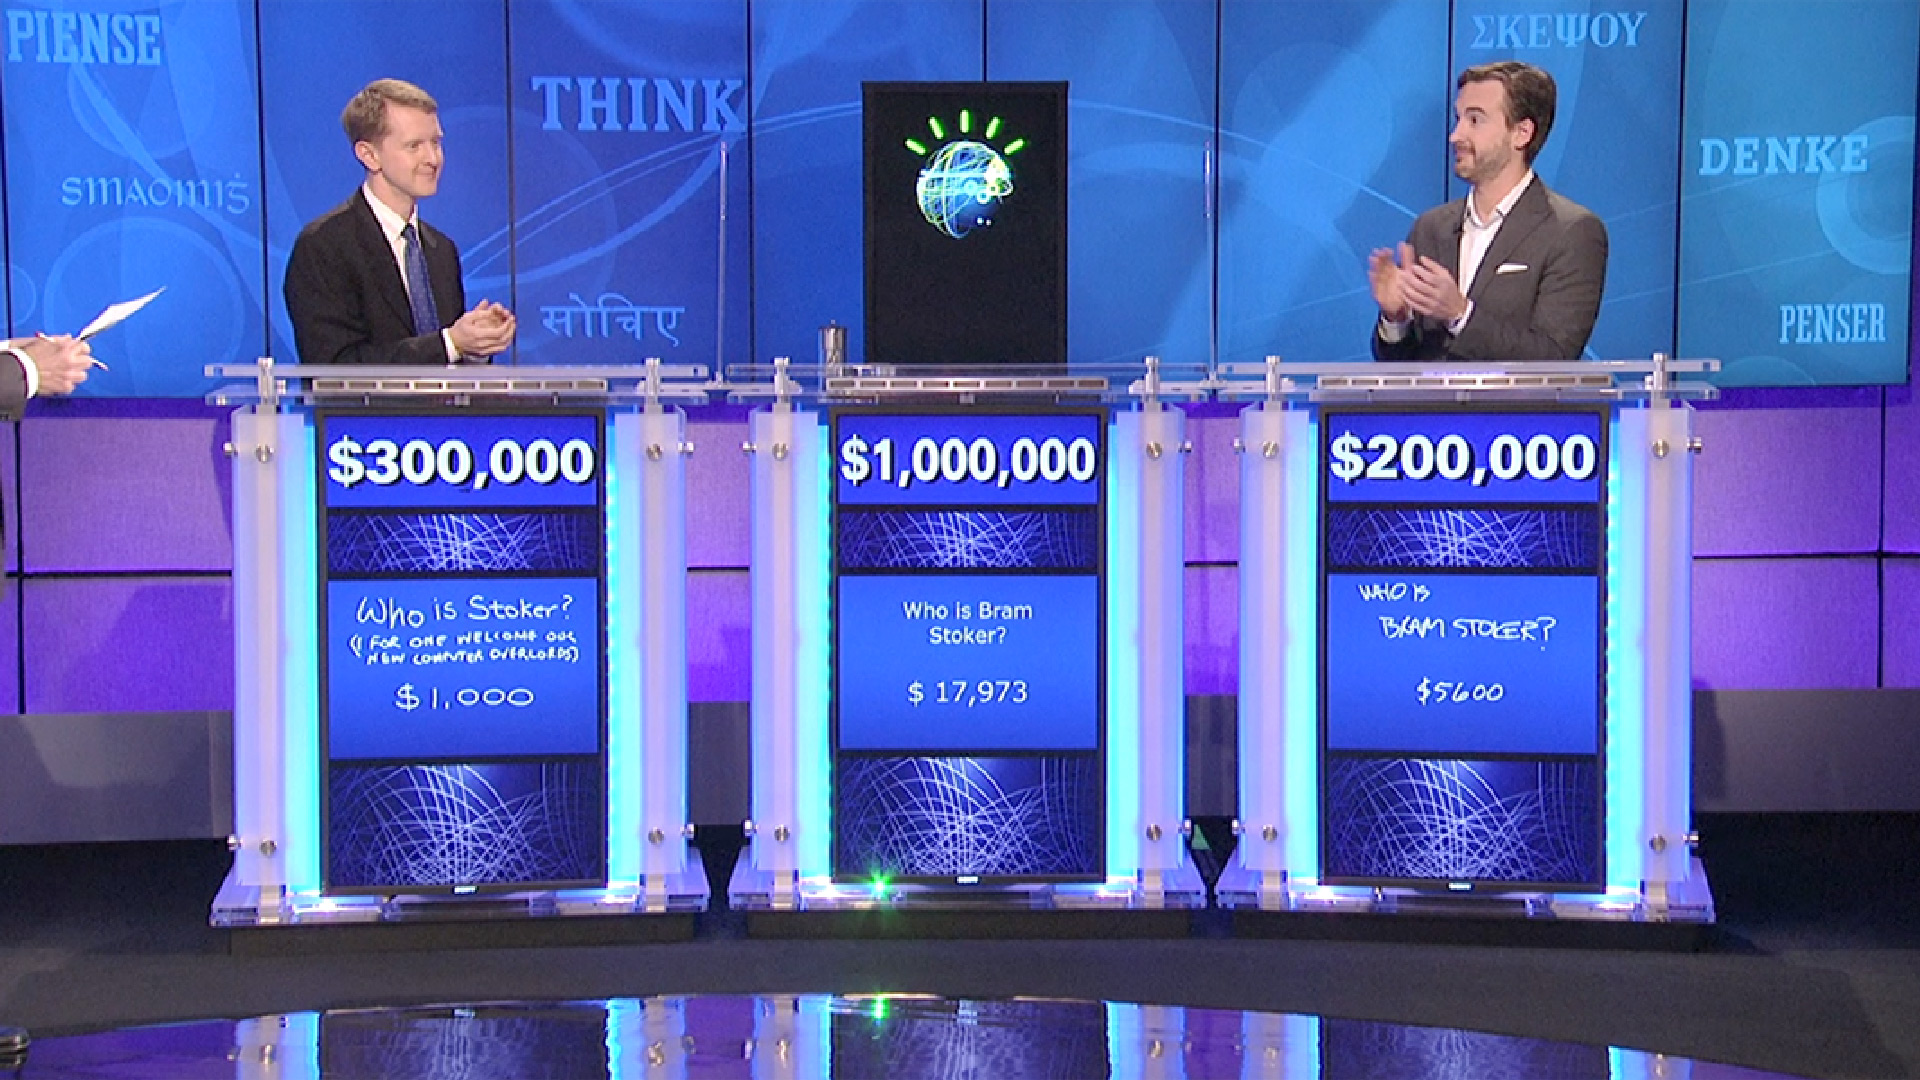
\includegraphics[width=1.0\linewidth]{qb/jeopardy}
                \pause
                \vspace{-8cm}
         \begin{block}{This is {\bf not} Jeopardy \cite{ferruci-10}}
		\begin{itemize}
                        \item Jeopardy: must decide to answer {\bf once}, after
                          complete question
                        \item Quiz Bowl: decide after each word
		\end{itemize}

	\end{block}

\end{frame}


\begin{frame}{How to approach this problem \dots}

  \begin{columns}
    \column{.5\linewidth}
    \gfxq{guess}{0.8}
    \column{.5\linewidth}
    \gfxq{buzzer}{0.8}
  \end{columns}
  \pause
\end{frame}


\begin{frame}
	\frametitle{Humans doing Incremental Classification}

	\begin{itemize}
		\item Thousands of questions are written every year
		\item Large question databases
		\item Teams practice on these questions (some online, e.g. IRC)
		\item How can we learn from this?
	\end{itemize}

\end{frame}

\begin{frame}{}

  \begin{columns}
    \column{.5\linewidth}
        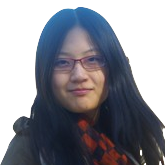
\includegraphics[width=0.7\linewidth]{general_figures/hehe} \\
        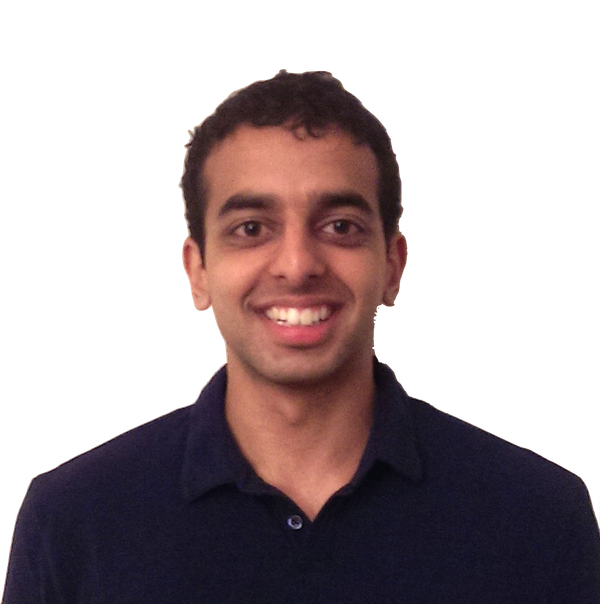
\includegraphics[width=0.7\linewidth]{general_figures/mohit}
    \column{.5\linewidth}
        \begin{block}{{\bf
              \href{http://cs.colorado.edu/~jbg//docs/qb_emnlp_2012.pdf}{Besting
                the Quiz Master: Crowdsourcing Incremental
                Classification Games}}}

          {\bf Jordan Boyd-Graber}, He He, and Hal {Daum\'{e} III}. \emph{Empirical Methods in Natural Language Processing}, 2012
        \end{block}

        \begin{block}{ {\bf \href{http://cs.colorado.edu/~jbg//docs/2014_emnlp_qb_rnn.pdf}{A Neural Network for Factoid Question Answering over Paragraphs}}}
\underline{\href{http://cs.umd.edu/~miyyer/}{Mohit Iyyer}}, {\bf Jordan Boyd-Graber}, Leonardo Claudino, Richard Socher, and Hal {Daum\'{e} III}.  \emph{Empirical Methods in Natural Language Processing}, 2014
        \end{block}


  \end{columns}
\end{frame}

\begin{frame}{Content Model}

\begin{block}{}
  \begin{center}
    \vspace{-.5cm}
    \begin{tabular}{cccc}
      \alert{content model} & oracle & policy & features \\
    \end{tabular}
    \vspace{-.5cm}
  \end{center}
\end{block}


  \begin{itemize}
   \item Bayesian generative model with answers as latent state
         \item Unambiguous Wikipedia pages
           \item Unigram term weightings (na\"ive Bayes, BM25)
    \item Maintains posterior distribution over guesses
    \item Always has a guess of what it should answer
      \begin{itemize}
        \item policy will tell us when to trust it
       \end{itemize}

  \end{itemize}
\end{frame}

\begin{frame}{Vector Space Model}

  \only<1>{\gfxq{unigram_models_0}{.8}}
  \only<2>{\gfxq{unigram_models_1}{.8}}
  \only<3>{\gfxq{unigram_models_2}{.8}}
  \only<4>{\gfxq{unigram_models_3}{.8}}
  \only<5>{\gfxq{unigram_models_4}{.8}}
  \only<6>{\gfxq{unigram_models_5}{.8}}
  \only<7>{\gfxq{unigram_models_6}{.8}}
  \only<8>{\gfxq{unigram_models_7}{.8}}
  \only<9>{\gfxq{unigram_models_8}{.8}}


\end{frame}



\begin{frame}{How can we do better?}

  \begin{itemize}
    \item Use relationship between questions (``China'' and
      ``Taiwan'')
    \item Use learned features and dimensions, not the words we start with
    \item Does the order of words matter?
  \end{itemize}

\end{frame}



\begin{frame}{Deep Averaging Networks}

  \only<1>{\gfxq{dan_1}{.8}}
  \only<2>{\gfxq{dan_2}{.6}}
  \only<3>{\gfxq{dan_3}{.6}}
  \only<4>{\gfxq{dan_4}{.6}}

\end{frame}




\begin{frame}{Training}

  \begin{columns}
    \column{.5\linewidth}
      \begin{itemize}
        \item Initialize embeddings from \textsc{word2vec}
        \item Randomly initialize composition matrices
        \item Update using \textsc{warp}
          \begin{itemize}
            \item Randomly choose an instance
            \only<2->{\item Look where it lands}
            \only<4->{\item Has a correct answer}
            \only<5->{\item Wrong answers may be closer}
            \only<6->{\item Push away wrong answers
            \item Bring correct answers closer}
          \end{itemize}
      \end{itemize}

    \column{.5\linewidth}

      \only<1>{\gfxq{warp_training_5}{.8}}
      \only<2>{\gfxq{warp_training_4}{.8}}
      \only<3>{\gfxq{warp_training_3}{.8}}
      \only<4>{\gfxq{warp_training_2}{.8}}
      \only<5>{\gfxq{warp_training_1}{.8}}
      \only<6>{\gfxq{warp_training_0}{.8}}
  \end{columns}

\end{frame}


\begin{frame}{Oracle}

\begin{center}
  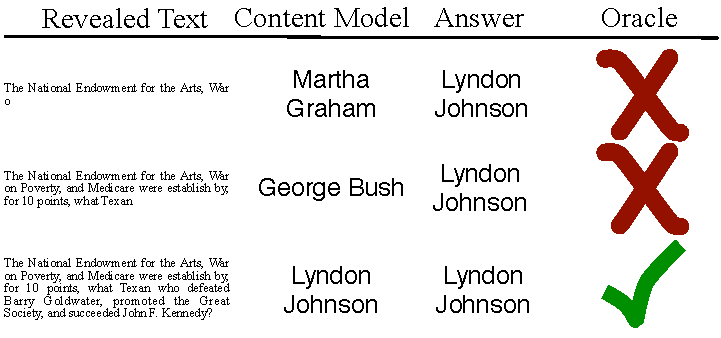
\includegraphics[width=0.8\linewidth]{qb/oracle}
\end{center}

\begin{itemize}
  \item As each token is revealed, look at content model's guess
    \item If it's right, positive instance; otherwise negative
      \item Nearly optimal policy to buzz whenever correct (upper bound)
\end{itemize}

\end{frame}

\begin{frame}{Policy}


 \begin{itemize}
    \item Mapping: state $\mapsto$ action
    \item Use oracle as example actions
    \item Learned as classifier \cite{langford-05}
    \item At test time, use the same features as for training
      \begin{itemize}
        \item Question text (so far)
        \item Guess
        \item Posterior distribution
        \item Change in posterior
      \end{itemize}
\end{itemize}

\end{frame}



\begin{frame}[plain]


\only<4->{\vspace{-.5cm}}

  \begin{columns}[T]
    \column{.3\linewidth}

    \only<1->{ 
\includegraphics[width=2\linewidth]{qb/feature_ex_l_1} \\ }
    \vspace{.5cm}
    \only<4->{ 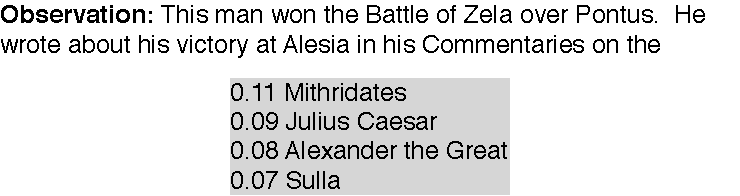
\includegraphics[width=2\linewidth]{qb/feature_ex_l_2}  \\ }
    \vspace{.5cm}
    \only<7->{ 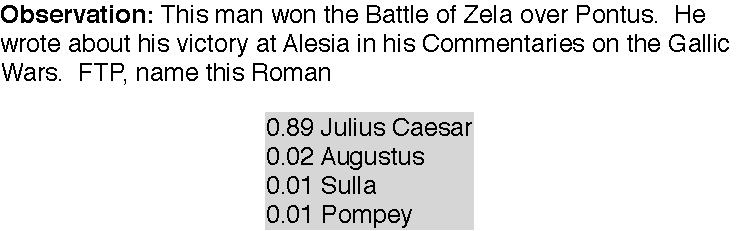
\includegraphics[width=2\linewidth]{qb/feature_ex_l_3}  \\ }


    \column{.68\linewidth}
    \vspace{-.5cm}
    \only<2->{ 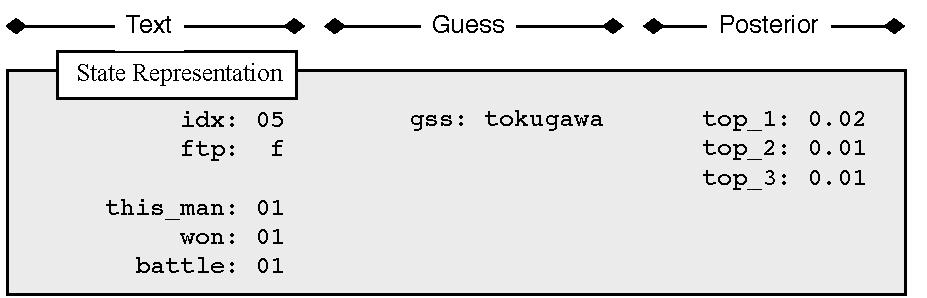
\includegraphics[width=.85\linewidth]{qb/feature_ex_r_1} \\ }
    \only<3->{ \vspace{-.5cm} \hspace{.5cm} 
\includegraphics[width=.1\linewidth]{qb/feature_ex_wait}  \\ }
    \only<5->{ 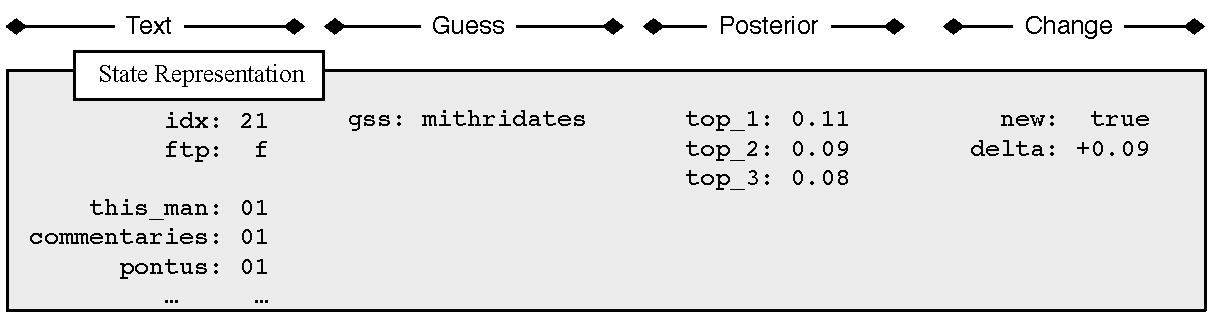
\includegraphics[width=\linewidth]{qb/feature_ex_r_2} \\ }
    \only<6->{ \vspace{-.5cm} \hspace{.5cm}
\includegraphics[width=.1\linewidth]{qb/feature_ex_wait}  \\ }
    \only<8->{ 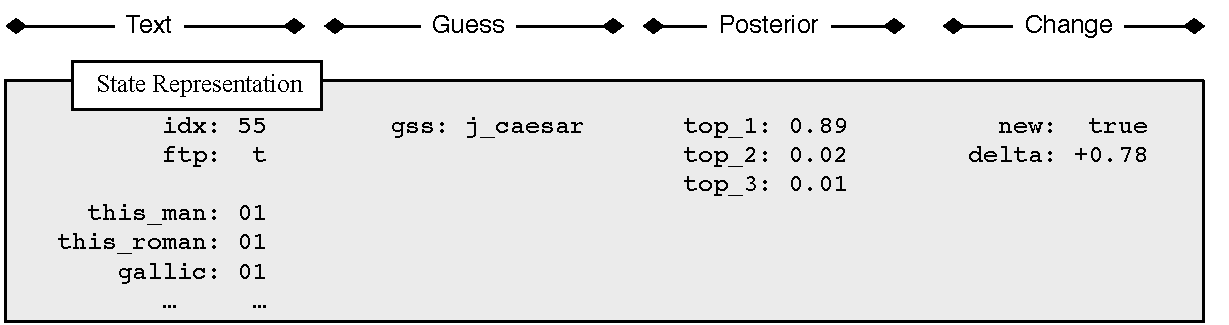
\includegraphics[width=\linewidth]{qb/feature_ex_r_3} \\ }
    \only<9->{ \vspace{-.5cm} \hspace{.5cm} 
\includegraphics[width=.1\linewidth]{qb/feature_ex_buzz}  \\ }
    \only<9->{Answer: {\bf Julius Caesar}}
  \end{columns}

\end{frame}



\begin{frame}
\frametitle{Interface}

\begin{columns}

	\column{0.5\linewidth}

	\begin{center}
		\includegraphics[width=0.8\linewidth]{qb/screenshot}
	\end{center}

	\column{0.5\linewidth}


	\only<2>{
	\begin{itemize}
		\item 7000 questions: first day
		\item 43000 questions: two weeks
		\item 461 unique users
                \item Imitated \dots
	\end{itemize}
        \gfxq{protobowl}{.8}
	}



\end{columns}
\end{frame}


\begin{frame}{Embedding}

  \gfxq{embedding}{1.0}

\end{frame}


\begin{frame}{Examining vectors}

  \only<1>{\gfxq{mann}{.65}}
  \only<2>{\gfxq{cabot}{.6}}

\end{frame}

\begin{frame}{Experiment 1}

		\begin{columns}
			\column{.25\linewidth}
				\gfxq{colby_jeo}{1.0}
                                Colby Burnett:
                                \$375,000
			\column{.25\linewidth}
				\gfxq{ben_jeo}{1.0}
                                Ben Ingram:
                                \$427,534
			\column{.25\linewidth}
				\gfxq{alex_jeo}{1.0}
                                Alex Jacobs: \$151,802
			\column{.25\linewidth}
				\gfxq{kristin_jeo}{1.0}
                                Kristin Sausville: \$95,201
		\end{columns}

                \pause


                \begin{center}
                End result: 200-200 tie!
                \end{center}

\end{frame}

\begin{frame}[plain]

\gfxq{hsnct1}{1.0}

\end{frame}

\begin{frame}{Experiment 2}

\gfxq{jennings}{.7}

\pause

\vspace{-5cm}
\gfxq{jennings_handshake}{1.0}

\end{frame}


\begin{frame}{Building on this Foundation}

\begin{itemize}
  \item More data helps
  \item Improving country pages specifically
  \item Still weak on popular culture
  \item Limited set of answers
\end{itemize}

\end{frame}

\begin{frame}[plain]

\only<1>{
\gfxq{seattle_crowd}{.5}
\gfxq{chicago_crowd}{.5}
}
\only<2>{
\gfxq{boring_dot_products}{1.0}
}

\end{frame}

% Diplomacy


\begin{frame}[plain]
\vspace*{-1pt}
\makebox[\linewidth]{\includegraphics[width=\paperwidth]{general_figures/black_box_compete}}
\end{frame}


% Update paper http://www.umiacs.umd.edu/~jbg/docs/
\begin{frame}{}

  \begin{columns}
    \column{.5\linewidth}
        \includegraphics[width=0.7\linewidth]{general_figures/vlad}
    \column{.5\linewidth}
        \begin{block}{{\bf
              \href{http://cs.colorado.edu/~jbg//docs/2015_acl_diplomacy.pdf}{Linguistic Harbingers of Betrayal: A Case Study on an Online Strategy Game}}}

          Vlad Niculae, Srijan Kumar, Jordan Boyd-Graber, and Cristian
          Danescu-Niculescu-Mizil. \emph{Association for Computational Linguistics}, 2015
        \end{block}

  \end{columns}
\end{frame}


\begin{frame}[plain]
\vspace*{-1pt}
\only<1>{\makebox[\linewidth]{\includegraphics[page=1,width=\paperwidth]{diplomacy/betrayal-slides}}}
\only<2>{\makebox[\linewidth]{\includegraphics[page=2,width=\paperwidth]{diplomacy/betrayal-slides}}}
\only<3>{\makebox[\linewidth]{\includegraphics[page=3,width=\paperwidth]{diplomacy/betrayal-slides}}}
\only<4>{\makebox[\linewidth]{\includegraphics[page=4,width=\paperwidth]{diplomacy/betrayal-slides}}}
\only<5>{\makebox[\linewidth]{\includegraphics[page=5,width=\paperwidth]{diplomacy/betrayal-slides}}}
\only<6>{\makebox[\linewidth]{\includegraphics[page=6,width=\paperwidth]{diplomacy/betrayal-slides}}}
\only<7>{\makebox[\linewidth]{\includegraphics[page=7,width=\paperwidth]{diplomacy/betrayal-slides}}}
\only<8>{\makebox[\linewidth]{\includegraphics[page=8,width=\paperwidth]{diplomacy/betrayal-slides}}}
\only<9>{\makebox[\linewidth]{\includegraphics[page=9,width=\paperwidth]{diplomacy/betrayal-slides}}}
\only<10>{\makebox[\linewidth]{\includegraphics[page=10,width=\paperwidth]{diplomacy/betrayal-slides}}}
\only<11>{\makebox[\linewidth]{\includegraphics[page=11,width=\paperwidth]{diplomacy/betrayal-slides}}}
\only<12>{\makebox[\linewidth]{\includegraphics[page=12,width=\paperwidth]{diplomacy/betrayal-slides}}}
\only<13>{\makebox[\linewidth]{\includegraphics[page=13,width=\paperwidth]{diplomacy/betrayal-slides}}}
\only<14>{\makebox[\linewidth]{\includegraphics[page=14,width=\paperwidth]{diplomacy/betrayal-slides}}}
\only<15>{\makebox[\linewidth]{\includegraphics[page=15,width=\paperwidth]{diplomacy/betrayal-slides}}}
\only<16>{\makebox[\linewidth]{\includegraphics[page=16,width=\paperwidth]{diplomacy/betrayal-slides}}}
\only<17>{\makebox[\linewidth]{\includegraphics[page=17,width=\paperwidth]{diplomacy/betrayal-slides}}}
\only<18>{\makebox[\linewidth]{\includegraphics[page=18,width=\paperwidth]{diplomacy/betrayal-slides}}}
\only<19>{\makebox[\linewidth]{\includegraphics[page=19,width=\paperwidth]{diplomacy/betrayal-slides}}}
\only<20>{\makebox[\linewidth]{\includegraphics[page=20,width=\paperwidth]{diplomacy/betrayal-slides}}}
\only<21>{\makebox[\linewidth]{\includegraphics[page=21,width=\paperwidth]{diplomacy/betrayal-slides}}}
\only<22>{\makebox[\linewidth]{\includegraphics[page=22,width=\paperwidth]{diplomacy/betrayal-slides}}}
\end{frame}

\begin{frame}[plain]
\vspace*{-1pt}
\only<1>{\makebox[\linewidth]{\includegraphics[page=1,width=\paperwidth]{diplomacy/betrayal-results}}}
\only<2>{\makebox[\linewidth]{\includegraphics[page=2,width=\paperwidth]{diplomacy/betrayal-results}}}
\only<3>{\makebox[\linewidth]{\includegraphics[page=3,width=\paperwidth]{diplomacy/betrayal-results}}}
\only<4>{\makebox[\linewidth]{\includegraphics[page=4,width=\paperwidth]{diplomacy/betrayal-results}}}
\only<5>{\makebox[\linewidth]{\includegraphics[page=5,width=\paperwidth]{diplomacy/betrayal-results}}}
\only<6>{\makebox[\linewidth]{\includegraphics[page=6,width=\paperwidth]{diplomacy/betrayal-results}}}
\only<7>{\makebox[\linewidth]{\includegraphics[page=7,width=\paperwidth]{diplomacy/betrayal-results}}}
\only<8>{\makebox[\linewidth]{\includegraphics[page=8,width=\paperwidth]{diplomacy/betrayal-results}}}
\only<9>{\makebox[\linewidth]{\includegraphics[page=9,width=\paperwidth]{diplomacy/betrayal-results}}}
\only<10>{\makebox[\linewidth]{\includegraphics[page=10,width=\paperwidth]{diplomacy/betrayal-results}}}
\only<11>{\makebox[\linewidth]{\includegraphics[page=11,width=\paperwidth]{diplomacy/betrayal-results}}}
\only<12>{\makebox[\linewidth]{\includegraphics[page=12,width=\paperwidth]{diplomacy/betrayal-results}}}

\end{frame}

\begin{frame}{}

  \begin{columns}
    \column{.5\linewidth}
      \includegraphics[width=.9\linewidth]{general_figures/an}
    \column{.5\linewidth}
        \begin{block}{{\bf
              \href{http://cs.colorado.edu/~jbg//docs/2015_acl_teaparty.pdf}{ Tea Party in the House: A Hierarchical Ideal Point Topic Model and Its Application to Republican Legislators in the 112th Congress}}}

          Viet-An Nguyen, Jordan Boyd-Graber, Philip Resnik, and Kristina Miler.  \emph{Association for Computational Linguistics}, 2015
        \end{block}

  \end{columns}

\end{frame}

% Commands for teaparty stuff
\newcommand{\subtwo}[2]{_{#1, #2}}
\newcommand{\subthree}[3]{_{#1, #2, #3}}
\newcommand{\minussubtwo}[2]{_{-{#1, #2}}}
\newcommand{\minussubthree}[3]{_{-{#1, #2, #3}}}
\newcommand{\suptwo}[2]{^{#1, #2}}
\newcommand{\supthree}[3]{^{#1, #2, #3}}
\newcommand{\minussuptwo}[2]{^{-{#1, #2}}}
\newcommand{\minussupthree}[3]{^{-{#1, #2, #3}}}
\newcommand{\prior}[1]{\mathcal{B}#1} % to be revised
\newcommand{\greentext}[1]{\textcolor{caribbeangreen}{#1}}
\newcommand{\yellowtext}[1]{\textcolor{amber}{#1}}
\newcommand{\redtext}[1]{\textcolor{red}{#1}}
\newcommand{\bluetext}[1]{\textcolor{blue}{#1}}

\providecommand{\gfx}[2]{
\begin{center}
	\includegraphics[width=#2\linewidth]{teaparty/figures/#1}
\end{center}
}



\frame{
\frametitle{Evaluation: Tea Party in the House}
    \begin{block}{The Tea Party}
    \small
    \begin{itemize*}
      \item American political movement for freedom, small government, lower tax
      \item Disrupting Republican Party and recent elections
      \item Organizations:
      \begin{itemize}
        \item Institutional: Tea Party Caucus
        \item Other: Tea Party Express, Tea Party Patriots, Freedom Works
      \end{itemize}
      \item ``\textbf{Conventional views of ideology as a single--dimensional, left–-right
          spectrum experience great difficulty in understanding or explaining the Tea Party.}''

        \hfill \cite[ARPS]{CarminesARPS15}
    \end{itemize*}
    \end{block}

    \vspace{-.2cm}
    \begin{block}{Goal}
    \small
    \begin{itemize*}
      \item Explain Tea Partiers in terms of issues and votes
      \item Identify Tea Partiers from their rhetoric
    \end{itemize*}
    \end{block}
}

\begin{frame}{Not everyone has a voting record}

  \begin{columns}
      \column{.25\linewidth}
        \gfx{carson}{.75}
        \gfx{fiorina}{.75}
      \column{.25\linewidth}
        \gfx{walker}{.75}
        \gfx{schwarzenegger}{.75}

    \column{.5\linewidth}
    \begin{itemize}
      \item Ideal points estimated based on voting record
      \item Not all candidates have a voting record
        \begin{itemize}
          \item Governors
          \item Entertainers
          \item CEOs
        \end{itemize}
        \pause
       \item But all politicians---by definition---talk
      \end{itemize}
  \end{columns}

\end{frame}


\begin{frame}{Let's use whatever data we have}

\begin{columns}
  \column{.6\linewidth}
  \gfx{carson_twitter}{.95}
  \column{.4\linewidth}
  A single model that uses:
  \begin{itemize}
    \item Bill text
    \item Votes
    \item Commentary
  \end{itemize}
  to map political actors to the same continuous space.
  \pause
  This work: congressional floor speeches
\end{columns}
\end{frame}

\section{Hierarchical Ideal Point Topic Model}


\frame{
    \frametitle{Hierarchical Ideal Point Topic Model: Intuition}
    \centering
    What are your thoughts on the issue of {\bf immigration}?
    \begin{figure}
    \centering
      \includegraphics[width=\textwidth]{teaparty/figures/framing}
    \end{figure}
}

\frame{
    \frametitle{Hierarchical Ideal Point Topic Model: Overview}
    \only<1-5>{
    \begin{block}{Using both votes and text to learn}
        \begin{itemize}
          \item Two-level topic hierarchy:
            \only<2>{
            \begin{itemize}
            \item \alert<2>{First-level nodes map to agenda issues}
            \item \alert<2>{Second-level nodes map to issue-specific frames}
	   \end{itemize}}
            \only<3>{\alert<3>{Use existing labeled data to learn priors for interpretable
                issues}}
            \only<4>{ \alert<4>{Ideal points for frames for predictions using text only}}

          \item\alert<5>{Ideal points in multiple interpretable dimensions}
        \end{itemize}
    \end{block}
    \vspace{-.5cm}
    \begin{figure}
      \centering
      \only<1>{\includegraphics[width=.9\textwidth]{teaparty/figures/s5/output_1}}%
      \only<2>{\includegraphics[width=.8\textwidth]{teaparty/figures/s5/output_2}}%
      \only<3>{\includegraphics[width=.9\textwidth]{teaparty/figures/s5/output_4}}%
      \only<4>{\includegraphics[width=.9\textwidth]{teaparty/figures/s5/output_5}}%
      \only<5>{\includegraphics[width=.9\textwidth]{teaparty/figures/s5/output_3}}%
    \end{figure}
    }

    \only<6>{
    \begin{block}{Hierarchical Ideal Point Topic Model: Inputs}
      \begin{itemize}
        \item A collection of votes $\{v \subtwo ab\}$
        \item A collection of $D$ speeches $\{\bm w_d\}$, each of which is given by legislator
            $a_d$
        \item A collection of $B$ bill text $\{\bm w'_b\}$
      \end{itemize}
    \end{block}
    \begin{center}
      \includegraphics[width=.75\textwidth]{teaparty/figures/s5/data}%
    \end{center}
    }
}

\frame{
    \frametitle{Hierarchical Ideal Point Topic Model}
    \only<1>{
    \begin{overlayarea}{\linewidth}{3.5cm}
    \begin{block}{Modeling bill text}
        \begin{itemize}
          \item Each bill text $b$ is a mixture over $K$ issues $\vartheta_b$
          \item Each bill token generated from topic at \redtext{first-level issue node}
        \end{itemize}
    \end{block}
    \end{overlayarea}
    \vspace{-1.2cm}
    \begin{center}
      \includegraphics[width=.8\textwidth]{teaparty/figures/s5/modeling_bills}
    \end{center}
    }

    \only<2>{
    \begin{overlayarea}{\linewidth}{3.5cm}
    \begin{block}{Hierarchical Ideal Point Topic Model: Generative Process}
        \begin{itemize}
          \item Each speech $d$ also has a distribution $\theta_d$ over $K$ issues
          \item Each issue $k$, each speech $d$ has distribution over frames $\psi \subtwo dk$
          \item Each speech token from topic at \redtext{second-level frame
          node}
        \end{itemize}
    \end{block}
    \end{overlayarea}
    \vspace{-1cm}
    \begin{center}
      \includegraphics[width=.8\textwidth]{teaparty/figures/s5/modeling_speeches}
    \end{center}
    }

    \only<3->{
    \begin{overlayarea}{\linewidth}{3.5cm}
    \begin{block}{Hierarchical Ideal Point Topic Model: Modeling votes}
        \begin{itemize}
          \item Legislator $a$ votes `Yea' on bill $b$ with probability $p(v \subtwo ab = \mbox{Yea}) = \Phi(x_b \sum_{k=1}^K \vartheta \subtwo bk \alert<4>{u \subtwo ak} +
          y_b)$
          \item \alert<3>{Ideal point} $\alert<5>{u \subtwo ak} \sim \mathcal{N}(\sum_{j=1}^{J_k} \alert<7>{\eta \subtwo kj} \alert<6>{\psi \subthree akj}, \rho)$
        \end{itemize}
    \end{block}
    \end{overlayarea}
    \vspace{-1cm}
    \begin{center}
      \includegraphics[width=.8\textwidth]{teaparty/figures/s5/modeling_idealpoint}
    \end{center}
    }
}


\section{Predicting Membership}

\frame{
    \frametitle{Tea Party Caucus Membership Prediction}
    \begin{block}{Experiment setup}
    \begin{itemize}
    \small
      \item Task: Binary classification of whether a legislator is a member of the Tea Party Caucus
      \item Evaluation metric: AUC-ROC
      \item Classifier: SVM$^{light}$
      \item Five-fold stratified cross-validation
    \end{itemize}
    \end{block}

    \pause

    \begin{block}{Features}
    \begin{itemize}
    \small
      \item Text-based features: normalized term frequency (\textbf{TF}) and \textbf{TF-IDF}
      \item \textbf{Vote}: binary features
      \item \textbf{HIPTM}: features extracted from our model including
      \begin{itemize}
        \item $K$-dim ideal point $u \subtwo ak$ estimated from both votes and text
        \item $K$-dim ideal point estimated from text only $\bm \eta_k^T \hat{\bm \psi} \subtwo ak$
        \item $B$ probabilities estimating $a$'s votes $\Phi(x_b \sum_{k=1}^K \vartheta \subtwo bk u \subtwo ak +
          y_b)$
      \end{itemize}
    \end{itemize}
    \end{block}
}

\frame{
    \frametitle{Tea Party Caucus Membership Prediction: Votes \& Text}
    \begin{center}
        \includegraphics<1>[width=\textwidth]{teaparty/figures/s5/votetext_1}
        \includegraphics<2>[width=\textwidth]{teaparty/figures/s5/votetext_2}
        \includegraphics<3>[width=\textwidth]{teaparty/figures/s5/votetext_3}
        \includegraphics<4>[width=\textwidth]{teaparty/figures/s5/votetext_4}
        \includegraphics<5>[width=\textwidth]{teaparty/figures/s5/votetext_5}
        \includegraphics<6>[width=\textwidth]{teaparty/figures/s5/votetext_6}
    \end{center}
}

\frame{
    \frametitle{Tea Party Caucus Membership Prediction: Text Only}
      \begin{center}
        \includegraphics<1>[width=\textwidth]{teaparty/figures/s5/textonly_1}
        \includegraphics<2->[width=\textwidth]{teaparty/figures/s5/textonly_2}
      \end{center}

%      \begin{block}{}
%        Vote-based features are not needed at test time, so this model makes it possible to do better
%prediction even for people who have no voting record in Congress
%        \begin{itemize}
%          \item e.g., new members of Congress or political candidates.
%        \end{itemize}
%      \end{block}
}



\frame{
    \frametitle{Multi-dimensional Ideal Points}
    \begin{figure}
      \centering
        %\includegraphics<1>[width=.7\textwidth]{teaparty/figures/s5/multdim_ip_112}%
        \includegraphics<1->[width=\textwidth]{teaparty/figures/s5/mult_ip_top}%
    \end{figure}

        \begin{block}{}
           Most highly polarized dimensions are about government spending
        \end{block}

}


\section{How They Talk}

\begin{frame}{Framing Healthcare}
	\gfx{health}{.8}
\end{frame}

\begin{frame}{Framing Macroeconomics}
	\gfx{macroeconomics}{.8}
\end{frame}


\begin{frame}{Polarization}
	\only<1>{\gfx{polarization_1}{.7}}
	\only<2>{\gfx{polarization_2}{.7}}
	\only<3>{\gfx{polarization_3}{.7}}
	\only<4>{\gfx{polarization_4}{.7}}
\end{frame}

\section{Conclusions}

\begin{frame}{Conclusion}

  \begin{itemize}
    \item Interpretability: topic models
    \item Intuitive trainability: games, translation
    \item Transparency
    \item Relevance
  \end{itemize}

\end{frame}

% \frame{
%   \frametitle{But wait, there's more!}

%   \vspace{-.5cm}

% \begin{columns}



%   \column{.5\linewidth}

%    \begin{block}{Computational Social Science}
%      \centering
%      \includegraphics[width=0.9\linewidth]{teaparty/figures/framing} \\
%      \cite{nguyen-13b,nguyen-15}
%    \end{block}


%     \begin{block}{Interactive Machine Learning}
%      \centering
%         \includegraphics[width=0.4\linewidth]{interactive_topic_models/new_interface} \\
%        \cite{boyd-graber-06b,ma-09,nikolova-09}
%     \end{block}


%   \column{.5\linewidth}


%     \begin{block}{Multilingual Topic Models}
%       \begin{center}
%         \begin{large}
%           $p_{\mbox{topic}}(e | f)$ \\
%          \end{large}
%       \cite{eidelman-12,hu-14}
%        \end{center}
%     \vspace{-.3cm}
%     \end{block}


%     \begin{block}{Sentiment / Internal State}
%     \centering
%         \includegraphics[width=0.4\linewidth]{general_figures/diplomacy} \\
%         \cite{niculae-15,sayeed-12,boyd-graber-10}
%     \end{block}




% \end{columns}

% }



\frame{

	\frametitle{Thanks}

        \begin{block}{Collaborators}
          \textsc{naqt}, Hal Daum\'e III (UMD), Philip Resnik (UMD), Cristian
          Danescu-Niculescu-Mizil (Cornell), Leah Findlater (UMD), Kevin Seppi
          (BYU), Eric Ringger (BYU)
        \end{block}

	\begin{columns}

	\column{.5\linewidth}
        \begin{block}{Funders}
        \begin{center}
          \includegraphics[width=0.4\linewidth]{general_figures/nsf}
       \end{center}
        \end{block}

	\column{.5\linewidth}
        \begin{block}{Supporters}
        	\gfxq{naqt}{.4}
        \end{block}

        \end{columns}
}




\begin{frame}{References}
\bibliographystyle{style/acl}
\tiny
\bibliography{bib/journal-full,bib/jbg}
\end{frame}



\begin{frame}{Using Compositionality}

  \only<1-2>{\gfxq{rnn_11}{.8}}
  \only<3>{\gfxq{rnn_10}{.8}}
  \only<4>{\gfxq{rnn_9}{.8}}
  \only<5>{\gfxq{rnn_8}{.8}}
  \only<6>{\gfxq{rnn_7}{.8}}
  \only<7>{\gfxq{rnn_6}{.8}}

  \only<8>{\gfxq{rnn_recursive_1}{.8}}
  \only<9>{\gfxq{rnn_recursive_2}{.8}}
  \only<10>{\gfxq{rnn_recursive_3}{.8}}

  \only<11>{\gfxq{rnn_5}{.8}}
  \only<12>{\gfxq{rnn_4}{.8}}
  \only<13>{\gfxq{rnn_3}{.8}}
  \only<14>{\gfxq{rnn_2}{.8}}

\end{frame}

	

\begin{frame}
	\frametitle{Learning which Features are Useful}

	\begin{itemize}
		\item Use how humans these data as a prior for supervised maxent model~\cite{daume-04}
		\item Prior for label $a$ and feature $f$ is a function of the number of buzzes $b$ and tf-idf~\cite{salton-68}
\begin{equation}
  \left[ \vphantom{\frac{a}{b}}\alpha \alert<4>{\ind{ b(a,f) > 0}} + \beta \alert<3>{ b(a,f)} + \gamma
  \right] \alert<2>{\mbox{tf-idf}(a,f)} .
\label{eq:meanweight}
\end{equation}
		\begin{itemize}
			\item $\alpha$, $\beta$, and $\gamma = 0$: na\"ive zero prior
			\item $\alpha$ and $\beta = 0$: linear transformation of the mean
			\item $\alpha$ and $\gamma = 0$: number of buzzes times tf-idf value of the features
		\end{itemize}

	\end{itemize}

\end{frame}

\begin{frame}
	\frametitle{Using buzzes as a prior}

\begin{equation*}
  \left[ \vphantom{\frac{a}{b}}\alpha \ind{ b(a,f) > 0} + \beta b(a,f) + \gamma
  \right] \mbox{tf-idf}(a,f) .
\end{equation*}

\begin{center}
\begin{tabular}{cccccc}
Answers & Weighting & $\alpha$ & $\beta$ & $\gamma$ & Error\footnote{Buzz and tf-idf computed on training data; grid search on dev data; error on test data} \\
\hline
\multirow{5}{*}{100} & zero & - & - & - & 0.22 \\
& tf-idf & - & - & 8.3 & 0.08 \\
&  buzz-binary & 10.7 & - & - & {\bf 0.06} \\
&  buzz-linear & - &  1.1 & - & 0.10 \\
& buzz-tier & - & 1.6 & 0.5 & 0.07 \\
\hline
\end{tabular}
\end{center}
\end{frame}





\begin{frame}
	\begin{center}

\vspace{-.6cm}
\begin{figure}[tb]
\centering

\subfigure[Buzzes over all Questions]{
\includegraphics[width=0.6\linewidth]{qb/buzz_cloud}
\label{fig:buzz_cloud}
}

\subfigure[Wuthering Heights Question Text]{
\includegraphics[width=0.45\linewidth]{qb/wuthering_heights_question}
\label{fig:wh_question}
}
\subfigure[Buzzes on Wuthering Heights]{
\includegraphics[width=0.45\linewidth]{qb/wuthering_heights_buzz}
\label{fig:wh_buzz}
}
\end{figure}


	\end{center}

\end{frame}



\begin{frame}
	\frametitle{Accuracy vs. Speed}

	\begin{center}
	  \includegraphics[width=0.8\linewidth]{qb/accuracy_vs_speed}
	  \end{center}

\end{frame}

\begin{frame}{How we could translate a sentence}

\only<1>{\gfxs{example_3}{.9}}
\only<2>{\gfxs{example_4}{.9}}
\only<3>{\gfxs{example_5}{.9}}
\only<4>{\gfxs{example_6}{.9}}
\only<5>{\gfxs{example_7}{.9}}
\only<6>{\gfxs{example_8}{.9}}
\only<7>{\gfxs{example_9}{.9}}
\only<8>{\gfxs{example_10}{.9}}
\only<9>{\gfxs{example_11}{.9}}
\only<10>{\gfxs{example_12}{.9}}
\only<11>{\gfxs{example_13}{.9}}
\only<12>{\gfxs{example_14}{.9}}
\only<13>{\gfxs{example_15}{.9}}
\only<14>{\gfxs{example_16}{.9}}
\only<15>{\gfxs{example_17}{.9}}
\only<16>{\gfxs{example_18}{.9}}
\only<17>{\gfxs{example_19}{.9}}
\end{frame}




\end{document}
